%! Author = nate
%! Date = 2/3/22
% Preamble
\documentclass[12pt]{sdsu-thesis}

%% Packages
\usepackage{amsmath}
\usepackage{amsthm}
\usepackage{float}
\usepackage{longtable}
\usepackage[bf,labelsep=period,textfont=bf]{caption}
\usepackage[normalem]{ulem}
\usepackage[document]{ragged2e}
%
%
\theoremstyle{theorem}
%\newtheorem{theorem}{Theorem}[section]

%\theoremstyle{definition}
%\newtheorem{definition}{Definition}[section]

\newtheorem{theorem}    {Theorem}[chapter]
\newtheorem{corollary}  [theorem]{Corollary}
\newtheorem{definition} [theorem]{Definition}
\newtheorem{example}    [theorem]{Example}
\newtheorem{lemma}      [theorem]{Lemma}
\newtheorem{proposition}[theorem]{Proposition}
\newtheorem{remark}     [theorem]{Remark}

%\theoremstyle{remark}
%\newtheorem*{remark}{Remark}

\usepackage{amsfonts}
\usepackage{graphicx}
\graphicspath{
    {Plots}
}
\usepackage{hyperref}
\hypersetup{
    colorlinks=true,
    linkcolor=blue,
    filecolor=magenta,
    urlcolor=cyan,
    citecolor=red
}
%\usepackage{textcomp}
%\newcommand{\subtitle}[1]{%
%  \posttitle{%
%    \par\end{center}
%    \begin{center}\LARGE#1\end{center}
%    \vskip0.5em}%
%}
%
%\usepackage{datatool}% http://ctan.org/pkg/datatool
%\newcommand{\sortitem}[1]{%
%  \DTLnewrow{list}% Create a new entry
%  \DTLnewdbentry{list}{description}{#1}% Add entry as description
%}
%\newenvironment{sortedlist}{%
%  \DTLifdbexists{list}{\DTLcleardb{list}}{\DTLnewdb{list}}% Create new/discard old list
%}{%
%  \DTLsort*{description}{list}% Sort list
%  \begin{enumerate}%
%    \DTLforeach*{list}{\theDesc=description}{%
%      \item \theDesc}% Print each item
%  \end{enumerate}%
%}


% Title Page
%\begin{document}
%\title{\textbf{San Diego State University
%\\{\Large Department of Mathematics}}}
%\subtitle{Meshfree data driven scattered interpolation estimates of lyapunov exponents using optimized radial basis functions}
%\author{Nathanael J. Reynolds \\ \\
%        Advisor \\
%        Christopher W. Curtis}
% ======================================================================
% ======================================================================
% You definitely need to edit things BELOW this line
% ======================================================================
% ======================================================================

% Author name and the author name in upper case
% (FORMAT) Has to match university records, check if you have
% (FORMAT) full middle name, or middle initital on record.
\author{Nathanael J. Reynolds}


% Title of the thesis (all in upper case), use \\ for line breaks as
% usual, you can use up to 4 lines and make sure to set the counter
% titlelines to the number of lines you used.
%
% This is for the title page
%
\title{MESHFREE DATA DRIVEN SCATTERED INTERPOLATION ESTIMATES OF LYAPUNOV EXPONENTS USING OPTIMIZED RADIAL BASIS FUNCTIONS}
% Number of lines in the title, without setting this the title page
% will not be formatted properly
\setcounter{titlelines}{4}


% Heading style title, the number of lines can be different here then
% in titlelines and in fact the thesis manual requires that this be at
% most 3 lines long so only put at most 2 pagebreaks here.  This is
% for the abstract pages and the signature page.
%
% (FORMAT) Make sure that this title has the EXACT same words at the
% (FORMAT) title-page-title
%
\titleheading{MESHFREE DATA DRIVEN SCATTERED INTERPOLATION ESTIMATES OF LYAPUNOV EXPONENTS USING OPTIMIZED RADIAL BASIS FUNCTIONS}


% (FORMAT) The "degree" is set on three lines; select one of the
% following formats.  See DTM P.41
%
% Degree (MA-Math)
%\degreeONE{Master of Arts}
%\degreeTWO{in}
%\degreeTHREE{Mathematics}

% Degree (MS-Math)
%\degreeONE{Master of Science}
%\degreeTWO{in}
%\degreeTHREE{Mathematics}

% Degree (with Concentration)
\degreeONE{Master of Science in Applied Mathematics}
\degreeTWO{with a Concentration in}
\degreeTHREE{Dynamical Systems}

% Degree (dual, concurrent)
%\degreeONE{Master of Science in Applied Mathematics}
%\degreeTWO{and}
%\degreeTHREE{Master of Science in Theoretical Typography}


% ======================================================================
% If you need to change the word 'Thesis' use \thesisname{Blah} and if
% you need to change the middle line between \degree and \degreein on
% the titlepage to something other then 'in' use \inofand{of} to use
% 'of' for instance.  (This should not be necessary)
% ======================================================================


% Dates
\gradyear{2022}
% (Format) Term Year
\submitdate{Spring 2022}


% ======================================================================
% Thesis Committee
% ======================================================================
%
% Your committee chair (don't include titles as per the manual)
% (FORMAT) Do not include the institution ("SDSU") for local faculty
% (FORMAT) members; however, for external members DO include the
% (FORMAT) institution.
\committeechair{Christopher W. Curtis}
\committeechairdept{Department of Mathematics and Statistics}

% Second committee member
\committeesecond{Bowen Shen}
\committeeseconddept{Department of Mathematics and Statistics}

% Third (usually different department) committee member
\committeethird{Arlette Baljon}
\committeethirddept{Department of Physics}

% Document
\begin{document}
    \justifying
    % Title page
    % (FORMAT) Mandatory for SDSU thesis
    \maketitle

    % Signature page
    % (FORMAT) Mandatory for SDSU thesis
    \makesignature

    % Copyright page
    % (FORMAT) Mandatory for SDSU thesis
    \begin{copyrightpage}
      Copyright~\copyright~2022 \\
      by \\
      Nathanael J. Reynolds
    \end{copyrightpage}

    \begin{dedication}
      \vspace{3in}
      \centering
      For my mother, Laurie Reynolds, who has always supported me, Perri Gellman, for putting me down the road
            of mathematics, and the Puyallup Tribe of Indians whom without their financial support, this would not be possible.
    \end{dedication}

    \begin{epigraph}
      We are all apprentices in a craft where no one ever becomes a master.\\
      \begin{flushright}
        -- Ernest Hemingway
      \end{flushright}
    \end{epigraph}

    \begin{abstract}
      % This just inserts the the abstract.tex file
      % You insert your abstract in the space below.


This work develops a globally convergent, data driven algorithm for estimating the Lyapunov exponents of a dynamical system.
This work rigorously tests our algorithm with two dynamical systems: The Lorenz equation and the Rossler equation. Additionally
the algorithm is used to approximate the Lyapunov exponents of two additional dynamical systems, the Chua equation, and
the Li equation \textit{Li et al.} \cite{item:6}.
The time series used as data points for the dynamical system was obtained
by numerical integration with the fourth-order Runge-Kutta scheme. Our algorithm then interpolates the time series
using radial basis functions. Three basic functions\texttwelveudash Gaussian, multiquadrics, and inverse\texttwelveudash
were tested using our algorithm. The shape parameter of the basic function was optimized using an algorithm
developed by \textit{Rippa} \cite{item:3}.
Our interpolation algorithm is used to produce a numerical approximation of the given dynamical system's Jacobian.
The Lyapunov exponents of the system are calculated by performing a QR-decomposition on the Jacobian approximation. We conducted
several trials with Lorenz and Rossler by varying the simulation parameters $t$, $dt$, and nearest neighbors.
Our trials provided good approximations of the Lorenz Lyapunov exponents except for two trials where $t=90$ and one where $dt=0.1$.
Our algorithm also produced good approximations of the Lyapunov exponents for the Chua and Li equations. However, the
algorithm struggled providing accurate approximations of the minimal Lyapunov exponent for Rossler but provided
accurate approximations for Rossler's maximal Lyapunov exponenent.



    \end{abstract}

    \tableofcontents

    \listoftables

    \listoffigures

    \begin{acknowledgments}
      I would like to thank Dr. Curtis for guidance on this topic and his personal
      kindness, Dr. Shen for his expertise on the Lornenz system and
      providing resources and feedback for this thesis,
      Joe Diaz for his positivity and always being helpful no matter what the need was, Shashwat Sharan
      for his friendship and his help in getting me through tough classes,
      Andrew Tuma for giving me a sense of camaraderie through this thesis writing process,
      Jay Lago for always being there to answer questions about research, the
      applied mathematics graduate cohort of 2022 for fun times and being awesome,
      and last but not least the Department of Mathematics and Statistics for
      providing the education that ultimately made this thesis possible.
    \end{acknowledgments}

    % Note that if you want something in single space you can go back and
% forth between single space and normal space by the use of \ssp and
% \nsp.  If you want doublespacing you can use \dsp.  \nsp is normally
% 1.5 spacing unless you use the doublespace option (or savepaper
% option)
%
%(FORMAT) Usually you *don't* want to mess with the spacing for your
%(FORMAT) final version.  If you think/know that the thesis template
%(FORMAT) and/or thesis style file is incorrect/incomplete, PLEASE
%(FORMAT) contact the maintainer.  THANK YOU!!!

\chapter{INTRODUCTION}
\label{chap:intro}
% By labeling the chapter, I can refer to it later using the
% label. (\ref{chap:intro}, \pageref{chap:intro}) Latex will take care
% of the numbering.
      In 1963, Edward Lorenz made his famous discovery of chaos while studying atmospheric convection. Since Lorenz's discovery, chaos has been
      a cornerstone in the field of dynamical systems. Both natural and man-made systems can exhibit chaotic behavior
      so understanding them is of great importance to science. One of the ways to study chaotic systems is by their Lyapunov exponents.
      Lyapunov exponents are a measure of how quickly the trajectories of two distinct and arbitarily distant points
      on an attractor seperate. The Lyapunov exponent is a measure of how predictable a given dynamical system
      is and gives a measure of the attractor's entropy.\\

      The use of meshfree local regression methods have been used independently in statistics dating back to the 19th Century \cite{item:21}.
      The use of radial basis functions (RBFs) as a method for meshfree approximations finds its origin with applications
      for geodesy, geophysics, mapping, and meteorology (\cite{item:1}, pp.13). RBFs have found use in other fields such as
      finding numerical solutions to PDEs, computer graphics, signal and image processing, sampling theory, statistics,
      finance, and optimization (\cite{item:1}, pp.1).\\

      This thesis explores a data-driven method for estimating the Lyapunov exponents of a dynamical system. We call this method
      meshfree scattered data interpolation using radial basis functions (MSDI-RBF). The method works by obtaining
      time series data from a dynamical system via numerical integration and inputting the time series data into an interpolation matrix. Each matrix
      element contains a basic function (see \textsection\ref{sec:rbf}) where data points in time series and a shape parameter $\epsilon$ (see \textsection\ref{sub:2.2}),
      are taken as arguments of the function. The interpolation matrix elements use $\epsilon$ to find the best fit to the data.
      This thesis explores a method for finding an optimal $\epsilon$\texttwelveudash developed by \textit{Rippa} \cite{item:3}\texttwelveudash as we move along the attractor.
      This allows
      the interpolation matrix to adapt to changing conditions on the attractor. The interpolation matrix is used
      to calculate an estimate of the dynamical system's Jacobian matrix which is then used in a QR-decomposition
      method to calculate the system's Lyapunov exponents.\\

      This thesis explores dynamical systems with known equations and uses the fourth-order Runge-Kutta method to numerically integrate
      in order to obtain time series data. No experimental data from a physical dynamical system has been used
      in this work. However, as this method is data-driven, it can be used
      on experimental data where the underlying equations of the dynamical system are unknown. The method offers an approach
      with non-local (global) convergence to the data set. Four systems are studied in this work: the Lorenz equation, the Rossler equation,
      the Chua equation, the Li equation.\\

  \section{Dynamical Systems}

      Dynamical systems are the mathematics of the real world. They are used to study problems as diverse as:
      weather systems, traffic flow, star formation, stock market pricing, social media behavior, disease spread, population growth, chemical reactions, etc.
      Further reading on these topics can be found in \cite{item:16}\cite{item:2}. Dynamical systems can be represented
      as discrete or continuous systems, called \textit{maps} and \textit{flows} respectively. This thesis only
      works with flows. The curious reader can read further about maps in \cite{item:17}.
      A flow's trajectory is the path that the flow takes with the progression of time. The space in which trajectories
      are plotted is called the \textit{phase space}. Since any point can serve as an initial condition for the
      dynamical system, the phase space is completely filled with trajectories.\\

      A strange attractor attracts trajectories in the phase
      space onto them. However, trajectories are not attracted to a single point nor do trajectories on the attractor fall into
      periodicity. Trajectories on a strange attractor are space filling; they will visit all points
      within the attractor as $t\to\infty$ but they will not visit the same point twice.
      Strange attractors are inherently nonlinear phenomena
      and a dynamical system exhibiting strange attractor behavior is said to be chaotic as trajectories on the attractor
      meet the three requirements of chaos discussed in \textsection\ref{sec:chaos}.\\

      The dynamical systems studied in this work are presented in the sections below. These systems were chosen because all
      of them are able to exhibit chaotic behavior and some are quite famous; as such their properties are well established
      in the literature. Historical details about the attractors will be provided where relevant.
      Lorenz and Rossler are famous attractors in the field of dynamical systems and a natural starting point for this study.
      The Chua circuit is an application from physics. The signum switch is an attractor of personal interest to the author
      and was explored by \textit{Li, et al.}\cite{item:6}.\\

    \subsection{The Lorenz Equations}

          In 1963, the meteorologist Edward Lorenz was running a twelve equation weather simulation when he made
          a peculiar discovery. Resuming his calculations from the previous day, he wanted to continue calculating where the simulation had last left off,
          so he input a value from the previous day into the model. In order to save space, he rounded the six
          decimal places down to three. He then observed that his calculations diverged over time turning into something completely
          unrecognizability from the previous day. Lorenz had discovered that this weather model was chaotic.
          In order to better understand this phenomenon, Lorenz sought a simpler system that could replicate
          this same behavior. Studying a system developed by Barry Saltzman in 1962 \cite{item:25}\cite{item:26},
            he came up with a simplified system of three ordinary differential equations given by:

          \begin{equation}\label{eq:lorenz}
              \begin{align}
                  \dot{x}&=\sigma(y-x)\\
                  \dot{y}&=x(r-z)-y\\
                  \dot{z}&=xy-bz
              \end{align}
          \end{equation}

          While the equations were designed to model convection
          within a fluid, they also model an electric dynamo \cite{item:11} and the chaotic waterwheel \cite{item:11}(\cite{item:2}, pp.310-312).
          When plotted in phase space, these equations produce the famous butterfly wing phase plot (Figure \ref{fig:attr}a),
          which is apropos for the colloquial name of chaos, The Butterfly Effect.\\

        \subsection{The Rossler Attractor}

          In 1976, inspired by Lorenz, Rossler created a
          simple model for studying chaos \cite{item:12}, the Rossler attractor (Figure \ref{fig:attr}b). The system is defined as:
          \begin{equation}\label{eq:rossler}
              \begin{align}
                  \dot{x}&=-y-z\\
                  \dot{y}&=x+ay\\
                  \dot{z}&=b+z(x-c)
              \end{align}
          \end{equation}

          The system has only one equilibrium point and two of the equations involved are linear, making the system's eigenvalues
          easier to find.\\

    \subsection{The Chua Circuit}

          The Chua circuit is the simplest circuit that is capable of exhibiting chaotic behavior \cite{item:13}.
          The circuit was developed by Leon Chua in 1983. The purpose for developing the circuit was two-fold.
          First, researchers wanted to realistically model the Lorenz equations in order to demonstrate
          chaos as a robust physical phenomenon and not the result of numerical error \cite{item:13}. The second
          motivation was to show that the Lorenz equations were chaotic in a rigorous mathematical sense \cite{item:13}.
          This work uses the Chua equations as presented in \textit{Meador} \cite{item:8}:
          \begin{equation}\label{eq:chua}
              \begin{align}
                  \dot{x}&=\alpha(y-x-f(x))\\
                  \dot{y}&=x-y+z\\
                  \dot{z}&=-\beta y
              \end{align}
          \end{equation}
          \begin{equation}\label{eq:chua1}
              f(x) =
              \begin{cases}
                  bx - a + b \ \ \ &\text{for} \ \ \ x\geq 1\\
                  ax  &\text{for} \ \ \ -1<x<1\\
                  bx + a - b &\text{for} \ \ \ x\leq 1
              \end{cases}
          \end{equation}

          The Chua circuit was successful in its goals.
          In 1984, the following year, Matsumoto was able to numerically confirm the existence of chaotic
          attractors on the circuit \cite{item:13}\cite{item:14}. In 1985, Zhong and Ayrom experimentally observed
          chaotic attractors \cite{item:13}\cite{item:22} and in 1986 \textit{Chua et al.} rigorously proved chaos for
          the equations \cite{item:13}.\\

    \subsection{The Signum "Li" Switch} %fix equation spacing

          The signum switch is a circuit that was contructed and studied by \textit{Li et al.}\cite{item:6} Mathematically, the
          dynamical system is concise:
          \begin{equation}\label{eq:signum}
              \begin{align}
                  \dot{x}&=y-x\\
                  \dot{y}&=-z \ \text{sgn}(x)\\
                  \dot{z}&=x \ \text{sgn}(y) - a
              \end{align}
          \end{equation}

          The equations are derived from a dimensionless form of the Lorenz equations. Like Chua, the attractor
          has a piecewise defined element. Piecewise attractors are common for circuits due to their simplicity
          to construct \cite{item:6}. \textit{Li et al.} presents a four-dimensional version of this attractor
          in their work. This work only looks at the three-dimensional version of the attractor. This attractor
          has seen some interest in the music world as the company Nonlinearcircuits created a module for use
          in modular synthesizers based on the work in \textit{Li et al.}\\

        \begin{figure}[H]
            \centering
            \begin{tabular}{lcc}
                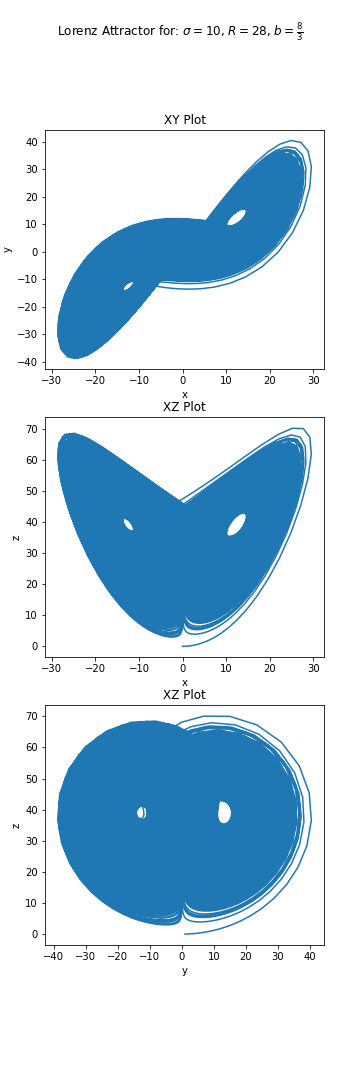
\includegraphics[width=8cm]{/Attractor Plots/3D Plots/Lorenz.png}&
                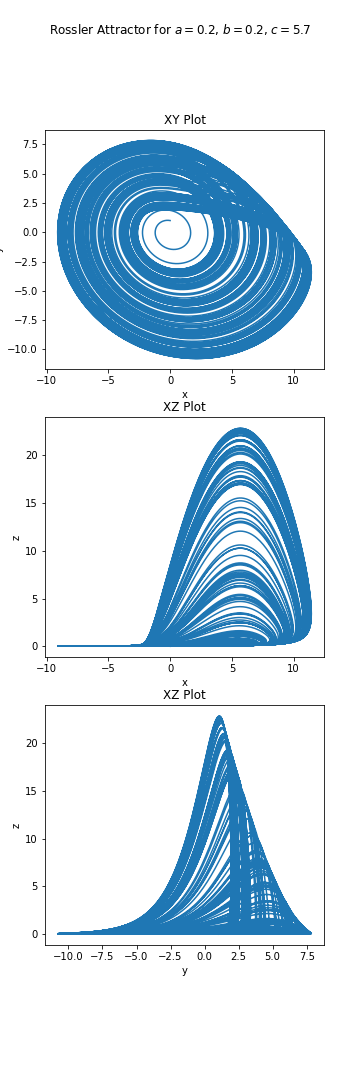
\includegraphics[width=8cm]{/Attractor Plots/3D Plots/Rossler.png}\\
                \hfil a &b\\
                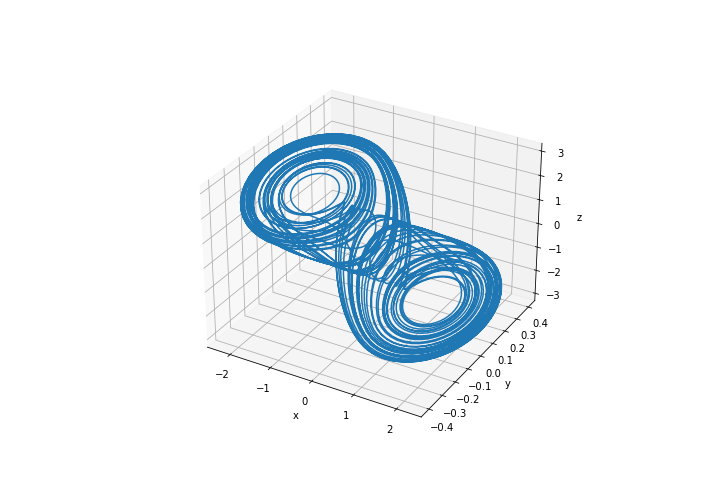
\includegraphics[width=8cm]{/Attractor Plots/3D Plots/Chua.png}&
                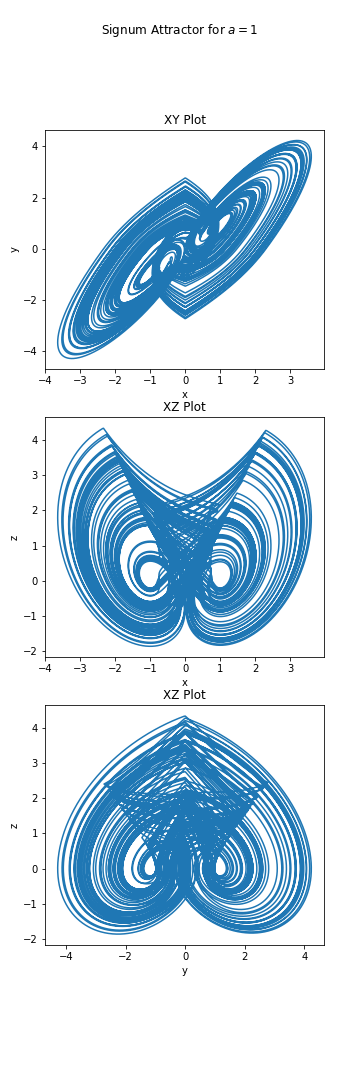
\includegraphics[width=8cm]{/Attractor Plots/3D Plots/Signum.png}\\
                \hfil c &d\\
            \end{tabular}
            \caption{a. Lorenz Attractor for $\sigma=10, \ r=28, \ b=\frac{8}{3}$, b. Rossler Attractor for $a=0.2, \ b=0.2, \ c=5.7$,
                c. Chua Attractor for $\alpha=9, \ \beta=\frac{100}{7}, \ a=-\frac{8}{7}, \ b=-\frac{5}{7}$, d. Li Attractor for $a=1$}\label{fig:attr}
        \end{figure}

`\section{Chaos}
  \label{sec:chaos}

      Chaos is the synthesis of the dialectic between, in a poetic sense, fate and free-will, between predetermination
      and an unknowable future. If one knows the initial state of a \textit{dynamical
      system}\texttwelveudash a system that changes over time\texttwelveudash with infinite precision, one is
      able to predict the time evolution of that system exactly from now until the heat
      death of the universe. However, in a chaotic system any infinitesimal perturbation in the measurement of this initial state will lead to
      drastically different futures for the perturbed system.\\

        While no universally accepted definition of chaos exists (\cite{item:2}, pp.331), there are agreed upon characteristics
        of chaotic systems:
        \begin{enumerate}
            \item The system must exhibit \textbf{aperiodic long-term behavior}. Trajectories never settle down to
                    fixed points, periodic orbits, or quasiperiodic orbits as $t\to\infty$.
            \item The system is \textbf{deterministic}. Irregular behavior arises from the system's nonlinearity rather
                    than any noisy driving forces. Generally speaking, there are no random or noisy input parameters.
            \item The system exhibits \textbf{sensitive dependence on initial conditions}. Nearby trajectories seperate
                    from each other exponentially fast.\\
        \end{enumerate}


  \section{Lyapunov Exponents}\label{sec:lyapunov}

      The motion on strange attractors exhibit sensitive dependence on initial conditions (see \textsection\ref{sec:chaos}).
      Lyapunov exponents are a measure of the exponential rates of divergence of neighboring
      trajectories on an attractor \cite{item:3}.
      To explore the concept more thoroughly consider a dynamical system:
      \begin{equation}\label{eq:lyu}
          \frac{d}{dt}\mathbf{y}=\mathbf{f}(\mathbf{y}), \ \mathbf{y}(0)=\mathbf{x}\in\mathbb{R}^n
      \end{equation}
      The affiliated flow map via the function is given by $\phi_t(\mathbf{x})$ so that $\mathbf{y}(t;\mathbf{x})=\phi_t(\mathbf{x})$.
      $\mathbf{f}(\mathbf{y})$ is called the velocity field (or vector field) of the flow. In this work $\mathbf{f}(\mathbf{y})$ will be
        referred to as the \textit{unknown function}. The unknown function corresponds to a data representation of the
        underlying differential equation expressions of the dynamical system. We will be interested in calculating the unknown function in order to
        generate numerical Jacobian approximations. To find the solution of $\mathbf{y}(t;\mathbf{x})$
      we first compute the Jacobian $J(t)$ where
      \begin{equation}\label{eq:jac}
          J(t)=D_y\mathbf{f}(\mathbf{y}(t;\mathbf{x}))
      \end{equation}
      An affilated time-dependent linear system can then be defined as
      \begin{equation}\label{eq:linsys}
          \frac{d\mathbf{U}}{dt}=J(t)\mathbf{U}, \ \mathbf(0)=\mathbf{I}
      \end{equation}
      Then the Lyapunov exponents are the eigenvalues of the matrix $\Lambda$ defined as
      \begin{equation}
          \Lambda=\lim\limits_{t\to\infty}\frac{1}{2t}\text{log}\mathbf{U}(t)\mathbf{U}^T(t)
      \end{equation}\\

      Lyapunov exponents give us a measure of how predictable the dynamical system is and a measure of entropy on the attractor. The presence of a positive
      Lyapunov exponent indicates sensitive dependence on initial conditions and is the telltale sign of chaos.
      However, dynamical systems can also have negative Lyapunov exponents which indicate no or contracting growth.\\

        \begin{remark}
            Exponential divergence of trajectories must stop when seperation distances are comparable to the diameter of the
            attractor (\cite{item:2}, pp.330). This phenomenon is called \textit{boundedness} and is an important concept
            to observe for chaotic systems. Dynamical systems such as $\dot{x}=ax$ also exhibit sensitive dependance on
            initial conditions (and have positive Lyapunov exponents). However, the aforementioned dynamical system is unbounded, nearby trajectories seperate
            from each other exponentially fast and become arbitarily distant from each other as $t\to\infty$. This latter property is not shared by
            chaotic attractors.
        \end{remark}

  %\subsection*{Numerical Methods}

          Lyapunov exponents are often difficult to compute analytically and thus are commonly solved with numerical
         methods. Several methods have been developed for numerically approximating Lyapunov exponents and are explored in the literature. Techniques
          for the calculation of exponents can either be done from analytic Jacobian calculations or be data driven. \textit{Eckmann et al.}
          develop a method for determining Lyapunov exponents from time series data with the use of Taken's Embedding
          Theorem \cite{item:18}. \textit{Wolf} introduces a method that utilizes Gram-Schmidt reorthonormalization \cite{item:4}.
          \textit{Deici et al.} uses QR-decomposition of the Jacobian of the dynamical system to estimate
          the Lyapunov exponents \cite{item:7}, \textit{Arbarbanel et al.} utilizes a similar OR-decomposition method but introduces a data
          driven method that uses Taylor series to approximate the Jacobian \cite{item:5}. This work also utilizes
        QR-decomposition to calculate Lyapunov exponents, details can be found in \textsection\ref{sec:lyuest}\\

  \section{Meshfree Scattered Data Interpolation using Radial Basis Functions}\label{sec:rbf}

          Mesh generation remains one of the most time consuming aspects of mesh-based numerical simulations such as:
      finite differences, finite elements, or finite volumes (\cite{item:1}, pp.1). These costs can be eliminated with
      meshfree methods as they rely on sets of independent points. Traditional numerical methods are often only suitable
      for low-dimensional systems (\cite{item:1}, pp.1). However, many real-world problems in science and engineering are high-dimensional
      problems that can often involve hundreds or thousands of variables. As such, applications for meshfree methods can
      be found in many different fields of study ranging from differential equations to machine learning.\\

      %\subsection*{Radial Basis Functions}

              The \textit{Gaussian} is a good first example of a \textit{basic function} to begin our discussion of radial basis functions (RBFs):
              \begin{equation}\label{eq:rbf}
                  \phi (r;\epsilon) = e^{-(\alpha r)^2}
              \end{equation}
              where $\alpha$ represents the \textit{shape parameter} (see \textsection\ref{sub:2.2}).
              RBFs are radially symmetric about their center and the shape parameter determines the flatness of the
              function. In order to build up a rigorous definition let
              \begin{equation}\label{eq:euc}
                  \gamma_k(\mathbf{x}) = \Vert \mathbf{x}-\mathbf{x}_k\Vert_2
              \end{equation}
              Then by $\phi(\gamma_k(\mathbf{x}))$ one can obtain for any fixed center $\mathbf{x}_k\in\mathbb{R}^s$ (\cite{item:1}, pp.17) a multivariate function
              \begin{equation}\label{eq:phi1}
                  \Phi_k(\mathbf{x};\epsilon)=\phi(\gamma_k(\mathbf{x}))=e^{-\alpha^2\Vert \mathbf{x}-\mathbf{x}_k\Vert_2^2}, \ \mathbf{x}\in\mathbb{R}^s
              \end{equation}
              where s is the dimension of the data space. This leads to a rigorous definition of radial function:
              \begin{definition}\label{def:1}
              A function $\Phi: \mathbb{R}^s\to \mathbb{R}$ is called $\textit{radial}$ provided there exists a
              $\textit{univariate}$ function $\phi:[0, \infty)\to\mathbb{R}$ such that
                  \begin{equation*}
                      \Phi({\mathbf{x})=\phi(\Vert \mathbf{x} \Vert)
                  \end{equation*}
              and $\Vert\cdot\Vert$ is some norm on $\mathbb{R}^s$ \texttwelveudash \ usually the Euclidean norm (\cite{item:1}, pp.17)}.
              \end{definition}

                  When $\phi(r)$ in definition \ref{def:1} is a basic function, we call it a radial basis function (RBF).
                  The $\Phi_k$ presented is a distance matrix. Using a radial basis function expansion
                  one is able to solve scattered data interpolation problems on $\mathbb{R}^s$ by assuming
                  \begin{equation}\label{eq:inter}
                      \mathcal{P}_f(\mathbf{x})=\sum_{k=1}^N c_k\phi(\gamma_k(\mathbf{x}))
                  \end{equation}
                  coefficients $c_k$ are found by solving the linear system
                  \begin{equation} \label{eq:dist}
                      \begin{bmatrix}
                          \phi(\Vert \mathbf{x}_1-\mathbf{x}_1\Vert_2) & \cdots & \phi(\Vert \mathbf{x}_1-\mathbf{x}_N\Vert_2) \\
                          \vdots & \ddots & \vdots \\
                          \phi(\Vert \mathbf{x}_N-\mathbf{x}_1\Vert_2) & \cdots & \phi(\Vert \mathbf{x}_N-\mathbf{x}_N\Vert_2)
                      \end{bmatrix}
                      \begin{bmatrix}
                          c_1 \\
                          \vdots \\
                          c_N
                      \end{bmatrix} =
                      \begin{bmatrix}
                          g(\mathbf{x}_1) \\
                          \vdots \\
                          g(\mathbf{x}_N)
                      \end{bmatrix}
                  \end{equation}

                  Where $g(\mathbf{x})$ represents a general test function. In this thesis we used $g(\mathbf{x})=\text{sinc}(\omega x_1)\text{sinc}(\omega x_2)\ldots\text{sinc}(\omega x_N)$ as the test function.
                    The work presented tests the scheme with several different RBFs. The basic functions used in the interpolator are presented
                  in Table \ref{table:2}.
                  \begin{table}
                          \centering
                          \begin{tabular}[h]{||c c||}
                              \hline
                              Name & $\phi$(r) \\ [0.5ex]
                              \hline
                              Gaussian & $e^{-\frac{r^2}{\epsilon^2}}, \ \epsilon>0$ \\
                              \hline
                              Multiquadric & $(r^2 + \epsilon^2)^{1/2}, \ \epsilon\geq 0$ \\
                              \hline
                              Inverse & $(r^2 + \epsilon^2)^{-1/2}, \ \epsilon\geq 0$ \\ [1ex]
                              \hline
                          \end{tabular}\\
                          \caption{Basic functions}\label{table:2}
                      \end{table}
\chapter{Methods}
\label{chap:methods}

        The following section details how the MSDI-RBF algorithm works and the conditions under which the algorithm was
        tested.
        There are several components to to MSDI-RBF algorithm and the following subsections will discuss each.
        The algorithm relies on QR-decomposition of the Jacobian to calculate Lyapunov exponents. As MSDI-RBF is
        data driven, we cannot rely on analytic methods to find the Jacobian. Therefore, we construct an interpolation
        matrix containing basic functions which take in as arguments time series data and a shape parameter $\epsilon$.
        The shape parameter must be optimized to find a best fit to the data in order to obtain the most accurate results.
        Linear algebraic operations are then performed to calculate the Jacobian.\\

    \section{Lyapunov Exponent Estimation}\label{sec:lyuest}
        \subsection{QR-Decomposition}

                In this work an algorithm developed by \textit{Deici et al.} \cite{item:7} is used in order to check the results
                of the MSDI-RBF. Deici's algorithm uses QR-decomposition of a dynamical system's
                Jacobian matrix in order to calculate the Lyapunov exponents. The method is not
                data driven and relies on calculations utilizing the exact Jacobian of the system computed from the dynamical system's differential equations.
                The work of this thesis also uses the QR-decomposition of the Jacobian. However, we use time series data fed into the MSDI-RBF algorithm in order to approximate the
                Jacobian matrix rather than doing calculations with the analytic Jacobian. A brief overview
                of the QR-algorithm developed by Deici is presented in this section. However, see \textit{Deici et al.} \cite{item:7} for a more comprehensive
                discussion.\\

                As an instructive example, consider the Lorenz system from equation (\ref{eq:lorenz}). In this work the following values
                were chosen for the parameters of the Lorenz system: $\sigma=10, \ r=28, \ b=\frac{8}{3}$. For a generic initial %change to canonical lorenz
                condition a general solution can be described by the flow map $\mathbf{y}(t)=\phi(t;\mathbf{x})$ where $\mathbf{x}=\{x_1, x_2,...,x_N\}$
                represents the initial condition. When numerically integrating using the 4th-order Runge-Kutta scheme,
                one obtains the famous Lorenz butterfly (Figure \ref{fig:attr}a).\\

                For a given solution of (\ref{eq:lorenz}) one can linearize the system (\ref{eq:linsys}) by computing the affiliated
                Jacobian, where
                \begin{equation}\label{eq:jaclor}
                    J(t) = \begin{bmatrix}
                            -\sigma & \sigma & 0 \\ r-z(t) & -1 & -x(t) \\ y(t) & x(t) & -b
                            \end{bmatrix}
                \end{equation}
                A approximation to the solution of (\ref{eq:lorenz}) is defined at discrete times $\{t_j \} _{j=0}^{N_T}$,
                $t=0$ and $t_j=j\delta t$. To generate an approximation to the Lyapunov exponents we solve
                \begin{equation}
                    \frac{d}{dt}{\bf U}_{j} = J(t){\bf U}_{j}, ~ {\bf U}_{j}(t_{j}) = {\bf Q}_{j}
                \end{equation}
                where ${\bf Q}_{0}={\bf I}$ and we perform a QR-decomposition such that
                \begin{equation}\label{eq:qr}
                    {\bf U}_{j}(t_{j+1}) = {\bf Q}_{j+1}{\bf R}_{j+1}
                \end{equation}
                The $m^{th}$ Lyapunov exponent, $\lambda_m$ is then given by
                \begin{equation}\label{eq:lyuest}
                    \lambda_{m} = \lim_{j\rightarrow \infty}\frac{1}{t_{j}}\sum_{k=1}^{j}\log  \left|({\bf R}_{k})_{mm} \right|
                \end{equation}\\
        \subsection{Computing Lyapunov exponents from data}

                \textit{Deici et al.'s} \cite{item:7} method is not a data driven method. It relies on the Jacobian obtained by linearizing
                the equations of a dynamical system equations. The knowledge of the underlying equations of a given dynamical
                system is a luxury not often had with real world dynamical systems. Instead, what is the researcher has are data
                points collected from an experimental system. Therefore, proposed in this work is a data driven method
                for calculating the Lyapunov exponents of a dynamical system.\\

                In \textit{Abarbanel et al.} \cite{item:5} the aforementioned problem is dealt with using least squares
                fitting to Taylor series expansions. This method is algorithmically unwieldy. Additionally, the accuracy
                of Taylor series expansions rely on proximity arguments which cannot be guaranteed to hold. Our method, MSDI-RBF,
                generates non-local (global) approximations to the map at each time step using nearest neighbors to
                a given point $\mathbf{y}(t_j)\equiv\mathbf{y_j}$. However, from \cite{item:5} our algorithm inherits
                \begin{enumerate}
                    \item {Use of a KD-tree algorithm. We find a list of the nearest neighbors $N_{nb}$, to the point
                            we wish to approximate $\mathbf{y}(t_j)$. We label the $l^{th}$ nearest neighbor of $\mathbf{y}_j$
                            as $\mathbf{y}_{l,j}^n$. While geometrically close to $\mathbf{y}_j$, $\mathbf{y}_{l,j}^n$
                            could correspond to a different time $t_k$. This set of points $\mathbf{y}_j\cup\{\mathbf{y}_{l,j}^n\}^{N_{nb}}_{l=1}$
                            is denoted as $\mathcal{I}_j$}
                    \item {We follow each nearest neighbor one time step, $\delta t$, forward in time generating the points
                            $\mathbf{y}_{j+1}$. Additionally, we generate $\mathbf{y}_{l,j}^{n,+}=\phi_{\delta t}}(\mathbf{y}_{l,j}^n)$
                            and $\mathbf{y}_{l,j}^{n,-}=\phi_{-\delta t}}(\mathbf{y}_{l,j}^n)$}
                    \item {Using second-order centered-finite differencing we obtain an approximation for the unknown
                            function $\mathbf{f}(\mathbf{y})$
                                \begin{equation*}
                                    \mathbf{f}_j=\frac{\mathbf{y}_{j+1}-\mathbf{y}_{j-1}}{2\delta t}, \
                                    \mathbf{f}_{l,j}^n=\frac{\mathbf{y}_{l,j}^{n,+}-\mathbf{y}_{l,j}^{n,-}}{2\delta t}
                                \end{equation*}}\\
                \end{enumerate}

        \subsection{Calculating the Jacobian}

                From this point our method diverges from \cite{item:5}. We use RBFs to build interpolatory aprroximations
                for the points $(y_j, f_j)$ and $\{(y_{l,j}^n, f_{l,j}^n)\}$. We can then differentiate
                to find approximations of $J(t)$. This section explores the algorithm used to calculate the approximated Jacobian $\tilde{J}(t)$.
                As stated prior, MSDI-RBF converges
                globally and can be used to generate analytic approximations to the map at each time step using the
                nearest-neighbors to a given point in $\mathbf{y}(t_j)$. The method produces a sequence of approximate Jacobians,
                $\tilde{J}_j=\tilde{J}(t_j)$. From time-step to time-step, we have the analytic formula for the matricies
                $\mathbf{U}_j$
                \begin{equation}\label{eq:u_anal}
                    \mathbf{U}_j(t_{j+1})=\mathbf{Q}_j+\int_{t_j}^{t_{j+1}}\tilde{J}(t)\mathbf{U}_j(t)dt
                \end{equation}
                The Trapezoid approximation scheme is used to get a stable approximation of (\ref{eq:u_anal})
                \begin{equation}
                    \left(\mathbf{I}-\frac{\delta t}{2}\tilde{J}_{j+1}\right)\mathbf{U}_j\left(t_{j+1}\right)=
                    \left(\mathbf{I}-\frac{\delta t}{2}\tilde{J}_{j}\right)\mathbf{Q}_j
                \end{equation}\\

                    In order to avoid transients, the first $\frac{50}{\delta t}$ points from the data set $\{\mathbf{y}_j\}_{j=0}^N$
                    are removed to produce the reduced data set $\mathbf{y}_{\text{red}}=\{\mathbf{y}_j\}_{j=50/\delta t}^N$.
                    A list of the neartest 50 neighbors $\mathbf{y}_{l,j}^n$ to every point on the trajectory $\mathbf{y}_{\text{red}}$ is then generated.
                    The data from $\mathbf{y}_{\text{red}}$ is placed into the distance matrix $\Phi$ represented by (\ref{eq:dist})
                    and an RBF is chosen to represent $\phi(r,\epsilon)$. The interpolation problem is then solved for $\mathbf{c}=[c_1,...,c_N]^T$.\\

                    Using our approximations $\mathbf{f}_j$ and $\{\mathbf{f}_{l,j}^n\}_{l=1}^{N_{nb}}$ over interpolation
                    points $\mathbf{y}_{\text{red}}$ and $\{\mathbf{y}_{l,j}^n\}_{l=1}^{N_{nb}}$ we find the RBF approximation $\mathbf{f}_m$ via
                    \begin{equation}
                        \mathbf{f}_m(\mathbf{y})=\sum_{l=0}^{N_{nb}}c_{ml}\phi(\Vert \mathbf{y}-\mathbf{y}_{l,j}^n\Vert_2)
                    \end{equation}
                    where $\mathbf{y}_{0,j}^n=\mathbf{y}_{j}$ and $m=\{1,...,n\}$. We find the approximation to the
                   Jacobian $D_{\mathbf{y}}\mathbf{f}(\mathbf{y})\vert_{\mathbf{y}=\mathbf{y}_{j}}}$ by finding gradients
                    \begin{equation}\label{eq:jacest}
                        \nabla_{\mathbf{y}}\mathbf{f}(\mathbf{y})\vert_{\mathbf{y}=\mathbf{y}_{j}}}=\sum\limits_{l=1}^{N_{nb}} c_{m,l}\phi'(\Vert \mathbf{y}-\mathbf{y}_{l,j}^n\Vert_2)\frac{\mathbf{y}-\mathbf{y}_{l,j}^n}{\Vert \mathbf{y}-\mathbf{y}_{l,j}^n\Vert_2}
                    \end{equation}
                    using (\ref{eq:jacest}) we are now able to perform QR-decomposition with (\ref{eq:qr}) and subsequently
                    calculate the estimates of the affiliated Lyapunov exponents using (\ref{eq:lyuest}).\\


    \section{Shape Parameter}\label{sub:2.2}

            The accuracy of many RBF schemes is dependent on a shape parameter $\epsilon$ (see Table \ref{table:2}). The $\epsilon$ value controls
            the steepness of the RBF. Generally when making approximations on data, the RBF should be made as flat as possible.
            However, nearly flat RBFs often cause the interpolation matrix to become near-singular. There is often an optimal
            $\epsilon$ for a corresponsing RBF on a given data set and this optimal $\epsilon$ is often found where in
            areas where the condition number is large.\\

    % Can discuss various methods of selecting ideal shape parameter

            There are several different methods for chosing an optimal shape parameter for an RBF. In this work an
            algorithm developed by \textit{Rippa} (\cite{item:1}, pp.146)\cite{item:3}. Other methods presented
            are by Faushauer (\cite{item:1}, pp.142-153) but will not be discussed in any detail in this work. Before discussing the optimization of
            $\epsilon$ however, we first look at the conditioning of matricies.\\

        \subsection{Condition Number}

                A matrix \textbf{A} is said to be singular if the det(\textbf{A})=0.
                Let \textbf{B} be an invertible matrix where det(\textbf{B})= 0 + $\eta$
                where $0<\eta<<1$. \textbf{B} is then said to be \textit{ill-conditioned}. These matricies
                are said to be \textit{near-singular}, meaning that small perturbations in the matrix elements can cause
                the matrix to become singular (\cite{item:19}, pp.114). Within numerical linear algebra, Ill-conditioned matricies
                can produce inaccurate results due to roundoff errors. However, it is not necessarily the case that
                results obtained from ill-conditioned matricies are inaccurate. However, the results cannot be trusted
                on their face without independent verification.\\

                The \textit{condition number} of a matrix is a measure of how ill-conditioned a matrix is and is given by
                \begin{equation}
                    \kappa(\mathbf{B})=\Vert\mathbf{B}\Vert\Vert\mathbf{B}^{-1}\Vert
                \end{equation}
                Singular matricies have an infinite condition number thus the larger the %define condition number better I guess?
                condition number of a matrix, the more ill-conditioned the matrix is. In trying to optimize $\epsilon$
                to obtain accurate results for our approximations, we face a contridiction: for large data sets, the optimal
                $\epsilon$ is often found for parameters where the interpolation matrix $\Phi$ is severely ill-conditioned (Figure \ref{fig:cond}).
                Thus, there is no guarantee that the scheme is stable for a given data set.
                \begin{figure}[h]
                    \centering
                    \begin{tabular}{lcc}
                        \includegraphics[width=6.5cm]{/Condition Number Plots/lorenz gaussian.png}&
                        \includegraphics[width=6.5cm]{/Shape Parameter/Lorenz, t=90.png}\\
                        \hfil a & b\\
                    \end{tabular}
                    \caption{a. Condition number vs. $\epsilon$ plot for Lorenz equation
                            b. Optimal shape parameter measured against time for Lorenz equation}\label{fig:cond}
                \end{figure}
                This feature is what is called the \textit{trade-off principle} (\cite{item:1}, pp.135-140). Faushauer identifies
                three trade-off principles
                \begin{enumerate}
                    \item \textbf{Accuracy vs. Stability}. The standard approach to solving RBF interpolation problems
                            has a conflict between theoretically achievable accuracy and numerical stability. If we use
                            $\epsilon$ to (exponentially) increase accuracy then the condition number also grows
                            exponentially.
                    \item \textbf{Accuracy and Stability vs. Problem Size}. The Contour-Pade algorithm solves the first
                            trade-off principle and is able to find an optimal $\epsilon$ without sacrificing accuracy
                            or stability. However, it comes at the expense of ability to deal with large data
                            sets. The details of this algorithm will not be discussed any further. The interested reader
                            may refer to (\cite{item:1}, pp.140)
                    \item \textbf{Accuracy vs. Efficiency}. This trade-off principle is associated with compactly supported
                            functions which will not be discussed further. Interested readers may refer to (\cite{item:1}, pp.140)
                \end{enumerate}
                In the following subsections, we discuss the method used in this thesis for finding an optimal $\epsilon$ to interpolate
                the attractor data using MSDI-RBF.\\

        \subsection{Trial and Error}

                The simplest method to choose a good shape parameter ($\epsilon$) is to run many experiments with different shape
                parameters and select the best one. This strategy can be effective if the underlying function generating
                the data is known since an error function can be generated (\cite{item:1}, pp.142). Without knowing the underlying
                function, it becomes difficult to determine what the best shape parameter value is. Additionally, if
                the data generating function is known, then the exercise of interpolating is pointless outside of
                academic examples.\\


                In this work\texttwelveudash and in study of dynamical systems generally\texttwelveudash the systems
                are capable of exhibiting chaotic behavior. The function of a chaotic attractor is almost
                never known. Additionally, underlying functions of real-world systems are also rarely known leaving this
                approach unsuitable for the our work.\\

        \subsection{LOOCV "Drop-One" Algorithm}

                \textit{Rippa} \cite{item:3} develops an algorithm to find an optimal $\epsilon$ value. This algorithm is used in this
                work. This algorithm works by taking a single data-point out of the data set, or dropping one, and interpolating
                to generate a point for the dropped data point. Then we perform
                a least-squares error fit on the dropped data set, comparing the error of the interpolated point in the
                'drop one' data set and the known point in the original data set (\cite{item:1}, pp.146). This algorithm is
                presented in this section. Rippa'a algorithm will be referred to as leave-one-out-cross-validation (LOOCV)\\

                To examine how this scheme works, consider the radial basis function interpolant $\mathcal{P}_f^{[k]}$ to the data
                $\{f_1,\ldots,f_{k-1},f_{k+1},\ldots,f_N\}$. From (\ref{eq:inter}) one arrives at interpolation problem
                \begin{equation}\label{eq:loocv}
                    \mathcal{P}_f^{[k]}(x)=\sum\limits_{j=1}^N c_j^{[k]}\phi(\gamma_k(x)), \ j\neq k
                \end{equation}
                where $\mathcal{P}_f^{[k]}(x_i)=f_i$ and $i=\{1,\ldots,k-1,k+1,\ldots,N\}$. $E_k$ represents the error between the original
                data set and the interpolated dropped point data set. $E_k$ is given by
                \begin{equation}\label{eq:error}
                    E_k=f_k-\mathcal{P}_f^{[k]}(x_k)
                \end{equation}
                This implementation of the algorithm using (\ref{eq:error}) is expensive (\cite{item:1}, pp.146). However, $E_k$ can be simplified into
                \begin{equation}
                    E_k = \frac{c_k}{\Phi_{kk}^{-1}}
                \end{equation}
                with $c_k$ representing the kth coefficient of $\mathcal{P}_f$. $\Phi_{kk^{-1}}$ represents the kth diagonal
                element of the inverse interpolation matrix. The derivation for this formula is given in \cite{item:3}. The
                quality of the fit is obtained from the norm of the error vectors $\mathbf{E}=[E_1,\ldots,E_N]^T$ obtained
                by removing one point from the original data and comparing the fit with the known removed value at the
                removed point (\cite{item:1}, pp.146). By looping over the shape parameter $\epsilon$, we can compare
                the error norms for different values of $\epsilon$ and choose the $\epsilon$ associated with the smallest
                error norm.\\

                The LOOCV algorithm has the advantage of not needing to know the function that generated the data, it
                works for large data sets, and its error bounds do not depend on the basic function.
                For this reason, the LOOCV method is a good algorithm for selecting an
                optimal $\epsilon$ and thus is used in this work.\\

    \section{Fill Distance}

            The attractors in this thesis have different geometries. To get a sense of how MSDI-RBF distributes data on
            the attractor,
            the fill distance is calculated. The fill distance can be understood as the pairwise distance between a
            set of evaluation points and the data set \textbf{y} and is given by
            \begin{equation}
                h=h_{\chi,\Omega}=\sup_{\substack{\mathbf{y}\in\Omega}} \min_{\substack{\mathbf{y}_j\in\chi}}\Vert \mathbf{y}-\mathbf{y}_j \Vert
            \end{equation}
            where $\chi$ is the data set and $\Omega$ is the domain. Faushauer creates a uniform grid in $\mathbb{R}^2$
            to create the grid to measure the fill distance (\cite{item:1}, pp.22). The data set worked with in (\cite{item:1}, pp.22)
            fills $\mathbb{R}^2$ as a scattered data set. This work is interested in spacing on the attractor and not
            all space in $\mathbb{R}^3$ so the same attractor calculated with a finer time step or longer simualtion time length
            is used in order to calculate the fill distances on the attractor.
            This thesis calculates fill distances as the trajectories move across the attractor.
            The fill distances calculated and plotted as a function of time.\\

\chapter{Results}
\label{chap:results}

            Presented in this section are the results of different experiments done with the MSDI-RBF. In this work, all of the dynamical systems were solved using the 4th-order Runge-Kutta method. The Lorenz and
            Rossler equations are used to stress test MSDI-RBF.
            We explore the effect that the time length of the simulation, $t$,
            has on the accuracy of MSDI-RBF approximations, the effect of the time step, $dt$, for the Runge-Kutta scheme, and the
            effect of the number of nearest neighbors $N_{nb}$.
            Additionally, final Lyapunov estimations from the MSDI-RBF scheme will be presented for the Chua and Li attractors.
            However, Chua and Li will not be used to explore the aforementioned parameter experiments. For all of the attractors
            we study the effect that the choice of RBF has on the accuracy of our approximations.\\

            The initial condition used for all systems was $\mathbf{x}_0\equiv(x, y, z) = (0, 1, 0)$. We tested Lorenz using its canonical
            parameter values $\sigma=28, \ r=40, \ b=\frac{8}{3}$. We tested Rossler using parameter values $a=0.2,b=0.2,c=5.7$.
            Chua tested using values $\alpha=9,\beta=\frac{100}{7},a=-\frac{8}{7},b=-\frac{5}{7}$ and Li used
            the parameter $a=1$. In general, the simulation run time $t=1000$, time step $dt=0.01$, nearest neighbors
            $N_{nb}=50$, and a Gaussian basic function were used as default simulation parameters which all other experiments were measured against.
            It should be assumed that the aforementioned simulation parameters are used unless otherwise specified.
            Optimal $\epsilon$ values were tested in the range (0,100]. The trace of the Jacobian was calculated for all systems
            where $tr(J(t))=\lambda_1+\lambda_2+\lambda_3$.\\

            The algorithm from \cite{item:7} was used to establish a baseline from which to measure the accuracy and precision
            of the MSDI-RBF algorithm and results are presented in Table \ref{table:deici}.
            \begin{table}
                \centering
                \begin{tabular}[h]{||c c c c c c c||}
                    \hline
                    Attractor & $t$ & $dt$ & $\lambda_1$ & $\lambda_2$ & $\lambda_3$ & $tr(J(t))$\\ [0.5ex]
                    \hline
                    Lorenz & 90 & 0.01 & 0.715488 &  0.0346102  &  -14.4151 & -13.6650\\
                    \hline
                    Lorenz & 500 & 0.01 & 0.869117 & 0.0078071 & -14.5432 & -13.6663\\
                    \hline
                    Lorenz & 1000 & 0.01 & 0.889032 & 0.0032922 & -14.5587 & -13.6664\\
                    \hline
                    Lorenz & 1000 & 0.1 & 0.465994 & 0.172585 & -11.4328 & -10.7942\\
                    \hline
                    Lorenz & 1000 & 0.05 & 0.886379 & 0.014464 & -14.4606 & -13.5598\\
                    \hline
                    Lorenz & 1000 & 0.005 & 0.881813 & 0.00477522 & -14.5532 & -13.6666\\
                    \hline
                    Lorenz & 1000 & 0.001 & 0.891902 & 0.00378951 & -14.5623 & -13.6666\\
                    \hline
                    Rossler & 180 & 0.01 & 0.0665055 & 0.0193292 & -5.47756 & -5.3917\\
                    \hline
                    Rossler & 1000 & 0.01 & 0.071127 & 0.0034966 & -5.41067 & -5.3360\\
                    \hline
                    Rossler & 2000 & 0.01 & 0.0716397 & 0.00127227 & -5.39827 & -5.3254\\
                    \hline
                    Rossler & 1000 & 0.1 & 0.0702216 & 0.0034646 & -5.24156 & -5.3370\\
                    \hline
                    Rossler & 1000 & 0.05 & 0.0718241 & 0.00270556 & -5.39934 & -5.3248\\
                    \hline
                    Rossler & 1000 & 0.005 & 0.0699829 & 0.00296756 & -5.40376 & -5.3308\\
                    \hline
                    Rossler & 1000 & 0.001 & 0.0723338 & 0.00249077 & -5.40338 & -5.3288\\
                    \hline
                    Chua    & 1000 & 0.01  & 0.32169   & 0.00143785 & -2.56737 & -2.2442\\
                    \hline
                    Li      & 1000 & 0.01 & 0.146263 & 0.00205924 & -1.14831 & -1\\[1ex]
                    \hline
                \end{tabular}\\
                \caption{Deici algorithm results}\label{table:deici}
            \end{table}\\

        \section{Lorenz Equation}

                We tracked the Jacobian error measured across the entire time series $\mathbf{y}$ (Figures \ref{fig:lorenzjac}, \ref{fig:lorenzjac3}, and \ref{fig:lorenzjac2}) and the
                affiliated optimal shape parameter as we move around the attractor (Figure \ref{fig:lorenzshape}).
                Jacobian errors were calculating using the equation
                \begin{equation}
                    \frac{\Vert \tilde{J}(t)-J(t) \Vert}{\Vert J(t) \Vert}
                \end{equation}
                Where $\tilde{J}(t)$ represents the approximated Jacobian, $J(t)$ respresents the exact Jacobian calculation at time $t$,
                and $\Vert\cdot\Vert_2$ is the Frobenius norm. The Lorenz equation was tested with simulation lengths $t=90$ and $t=1000$. Time-steps $dt=0.01$ and
                $dt=0.001$ were used in calculation for both simulations lengths. Additionally,
                we calculated Jacobian error estimates for, $t=500$ for $dt=0.01$, and $dt=0.1, \ 0.05, \ 0.005, \ 0.001$ for $t=1000$ (Figure \ref{fig:lorenzjac2}).
                Lyapunov estimations were made for the aforementioned parameters as well as number of nearest neighbors and
                multiquadric and inverse basic functions at $t=1000$ and $dt=0.01$ (Figure \ref{fig:lorenzjac3}).\\
            \begin{figure}[H]
                \centering
                \begin{tabular}{lcc}
                    \includegraphics[width=6.5cm]{/Jacobian Error/Lorenz, t=90.png}&
                    \includegraphics[width=6.5cm]{/Jacobian Error/Lorenz, t=90 dt=0,001.png}\\
                    \hfil a &b\\
                    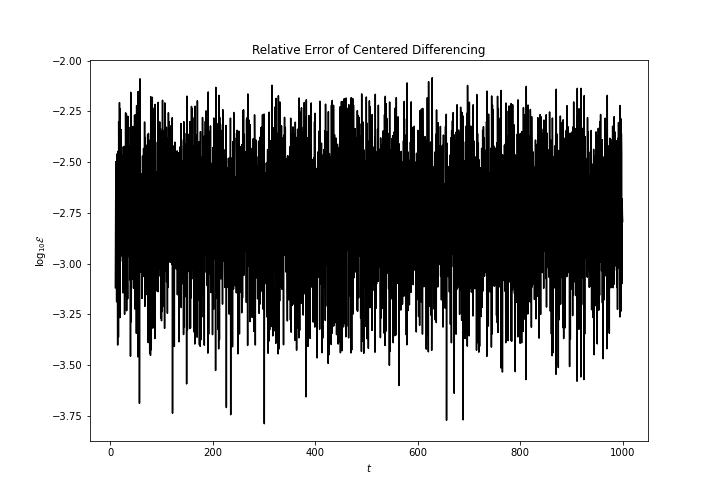
\includegraphics[width=6.5cm]{/Jacobian Error/Lorenz, t=1000.png}&
                    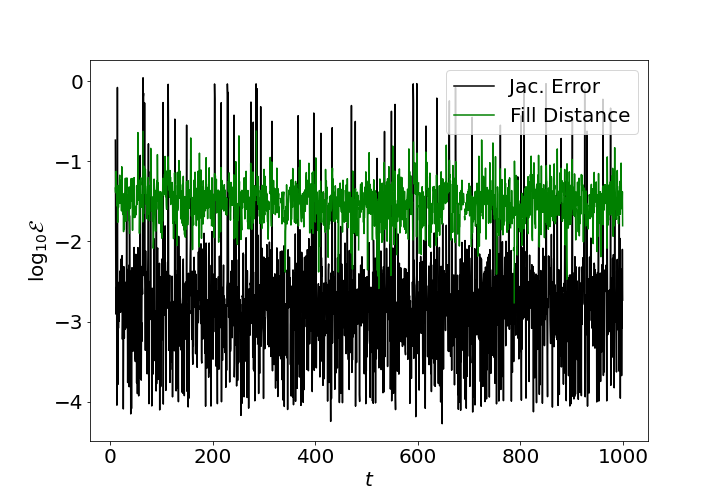
\includegraphics[width=6.5cm]{/Jacobian Error/Lorenz, dt=0,001.png}\\
                    \hfil c &d\\
                \end{tabular}
                \caption{Lorenz Jacobian Error and Fill Distance, a. $t=90$, $dt=0.01$ b. $t=90$, $dt=0.001$ c. $t=1000$, $dt=0.01$ d. $t=1000$, $dt=0.001$}\label{fig:lorenzjac}
            \end{figure}
            \begin{figure}[H]
                \centering
                \begin{tabular}{lcc}
                    \includegraphics[width=6.5cm]{/Shape Parameter/Lorenz, t=90.png}&
                    \includegraphics[width=6.5cm]{/Shape Parameter/Lorenz, t=90 dt=0,001.png}\\
                    \hfil a &b\\
                    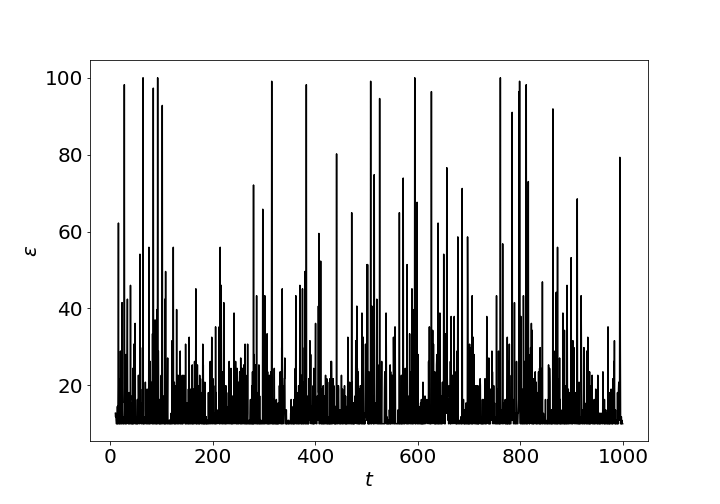
\includegraphics[width=6.5cm]{/Shape Parameter/Lorenz, t=1000 2.png}&
                    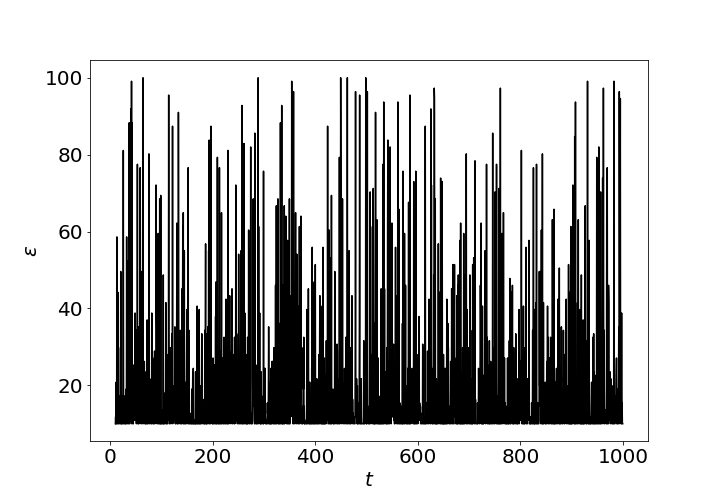
\includegraphics[width=6.5cm]{/Shape Parameter/Lorenz, t=1000 dt=0,001.png}\\
                    \hfil c &d\\
                \end{tabular}
                \caption{Lorenz shape parameter vs. time, a. $t=90$, $dt=0.01$ b. $t=90$, $dt=0.001$ c. $t=1000$, $dt=0.01$ d. $t=1000$, $dt=0.001$}\label{fig:lorenzshape}
            \end{figure}
            \begin{figure}[H]
                \centering
                \begin{tabular}{lcc}
                    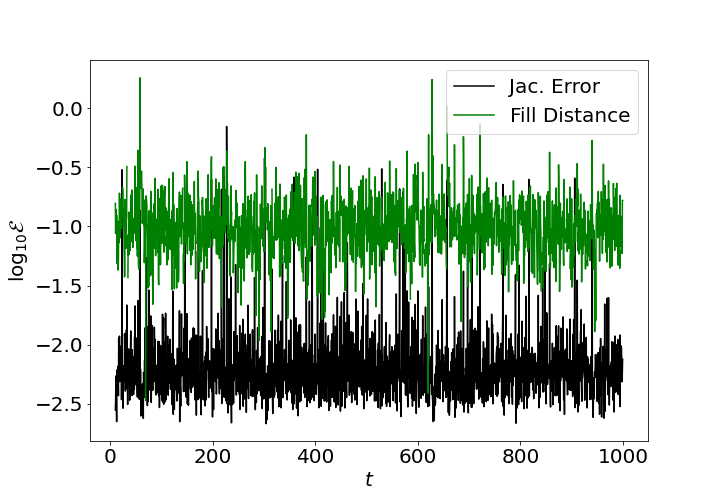
\includegraphics[width=6.5cm]{/Jacobian Error/Lorenz mult.png}&
                    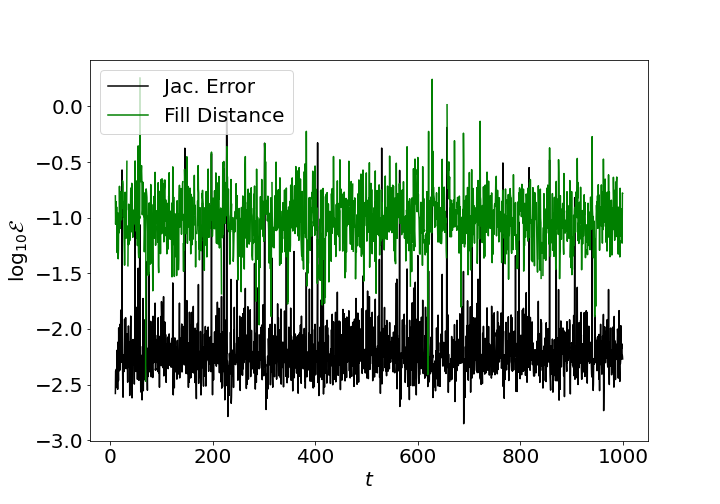
\includegraphics[width=6.5cm]{/Jacobian Error/Lorenz inv.png}\\
                    \hfil a &b\\
                    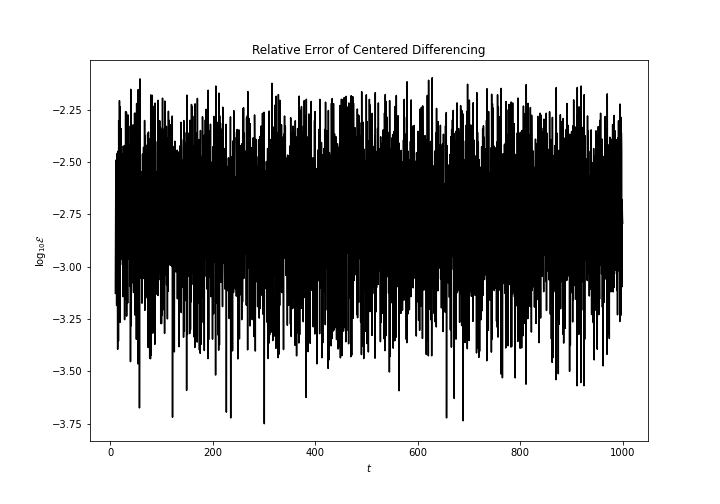
\includegraphics[width=6.5cm]{/Jacobian Error/Lorenz, 100nbrs.png}&
                    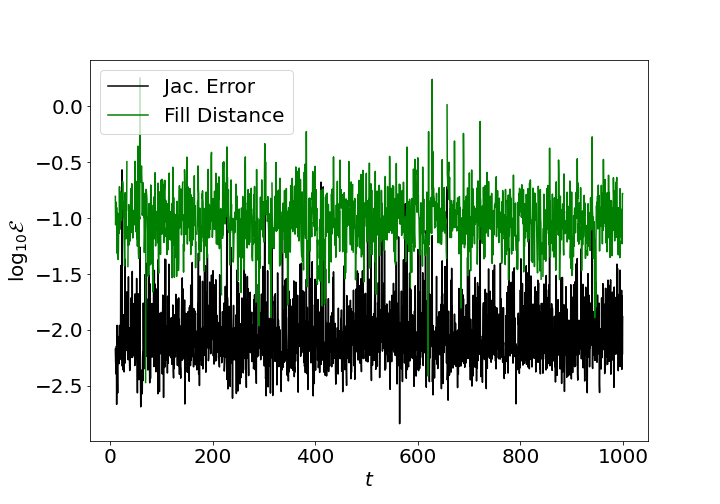
\includegraphics[width=6.5cm]{/Jacobian Error/Lorenz, 150nbrs.png}\\
                    \hfil c &d\\
                \end{tabular}
                \caption{Lorenz Jacobian Error and Fill Distance, a. multiquadric b. inverse c. $N_{nb}=100$ d. $N_{nb}=150$}\label{fig:lorenzjac3}
            \end{figure}

            \begin{table}
                \centering
                \begin{tabular}[h]{||c c c c c c c c||}
                    \hline
                    $\phi (x,\epsilon)$ & $t$ & $dt$ & $N_{nb}$ & $\lambda_1$ & $\lambda_2$ & $\lambda_3$ & $tr(\tilde{J}(t))$\\
                    \hline
                    gaussian & 90 & 0.01 & 50 & 0.647603 &   0.108388  &  -12.8713 & -12.1153\\
                    \hline
                    gaussian & 90 & 0.001 & 50 & 0.776243 & -0.0293548 & -8.41689 & -7.6700\\
                    \hline
                    gaussian & 500 & 0.01 & 50 & 0.755684 & 0.124363 & -14.3492 & -13.4692\\
                    \hline
                    gaussian & 1000 & 0.01 & 50 & 0.76659 & 0.129778 & -14.5085 & -13.6121\\
                    \hline
                    multiquadric & 1000 & 0.01 & 50 & 0.770113 & 0.125643 & -14.5009 & -13.6051\\
                    \hline
                    inverse & 1000 & 0.01 & 50 & 0.771143 & 0.124422 & -14.5006 & -13.6050\\
                    \hline
                    gaussian & 1000 & 0.01 & 100 & 0.763427 & 0.130108 & -14.5238 & -13.6303\\
                    \hline
                    gaussian & 1000 & 0.01 & 150 & 0.764278 & 0.131224 & -14.5234 & -13.6279\\
                    \hline
                    gaussian & 1000 & 0.1 & 50 & 2.87036 & -1.49536 & -20.4797 & -19.1047\\
                    \hline
                    gaussian & 1000 & 0.05 & 50 & 1.44894 & -0.465272 & -17.208 & -16.2243\\
                    \hline
                    gaussian & 1000 & 0.005 & 50 & 0.847037 & 0.0399775 & -14.3954 & -13.5084\\
                    \hline
                    gaussian & 1000 & 0.001 & 50 & 0.895842 & 0.000249988 & -14.1642 & -13.2681\\ [1ex]
                    \hline
                \end{tabular}\\
                \caption{MSDI-RBF Lyapunov Estimates for Lorenz equation}\label{table:lorenzest}
            \end{table}

        \section{Rossler Equation}

                We tested Rossler equation under the same parameter values as the Lorenz equation with one exception,
                the simulation run time of the Rossler tests were doubled from what was tested in Lorenz. However, the same procedure
                is followed.
                The Jacobian errors
                and fill distances measured against time are presented in Figure \ref{fig:rosslerjac}, \ref{fig:rosslerjac3}, and \ref{fig:rosslerjac2} and optimal shape parameters
                in Figure \ref{fig:rosslershape}. The Lyapunov
                exponent estimations are presented in Table \ref{table:rosslerest}.\\
            \begin{figure}[H]
                \centering
                \begin{tabular}{lcc}
                    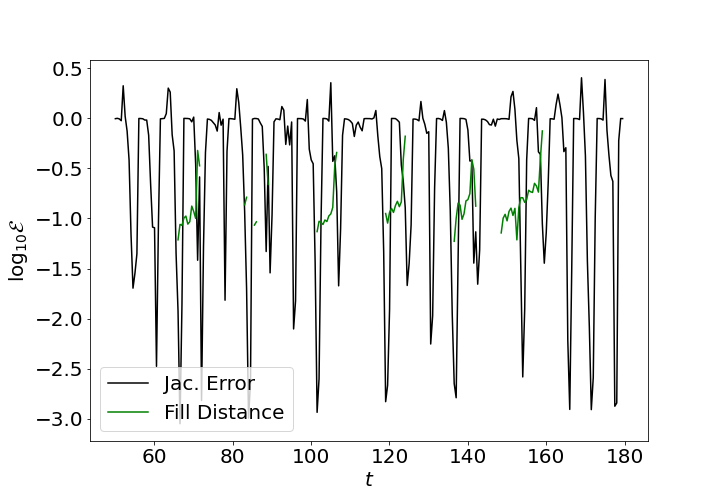
\includegraphics[width=6.5cm]{/Jacobian Error/Rossler, t=180.png}&
                    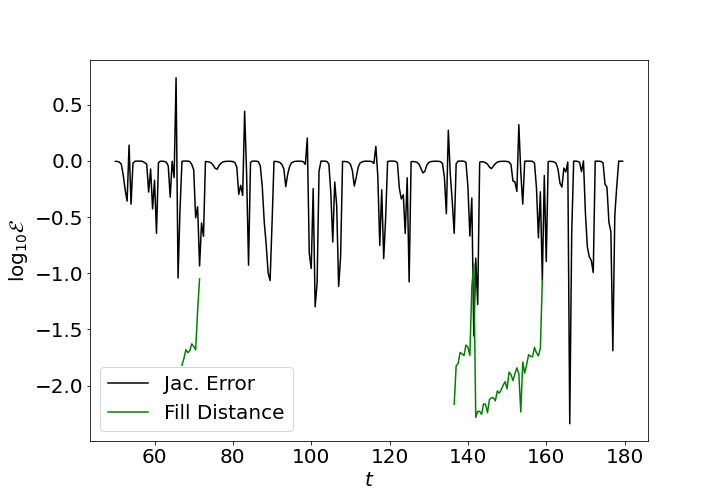
\includegraphics[width=6.5cm]{/Jacobian Error/Rossler, t=180 dt=0,001.png}\\
                    \hfil a &b\\
                    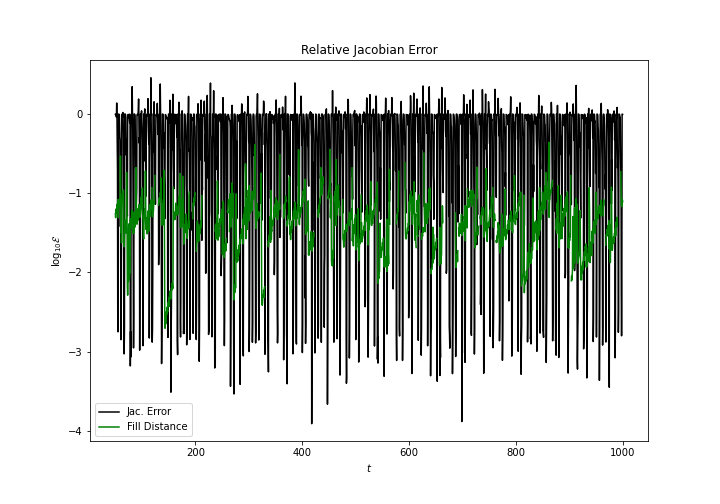
\includegraphics[width=6.5cm]{/Jacobian Error/Rosller, t=1000.png}&
                    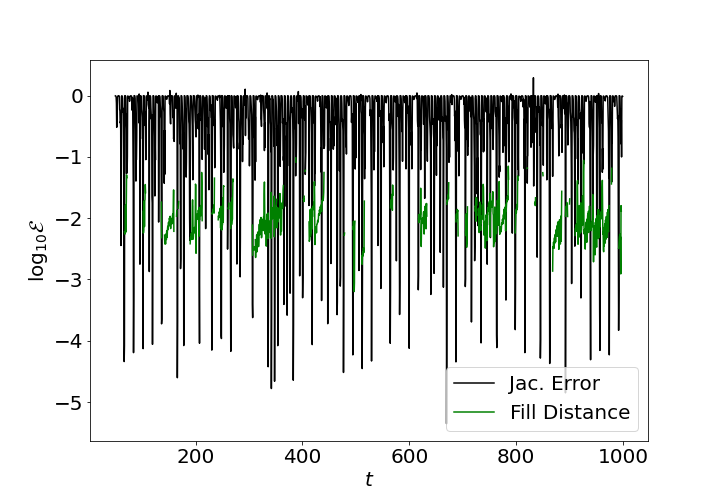
\includegraphics[width=6.5cm]{/Jacobian Error/Rossler, dt=0,001.png}\\
                    \hfil c &d\\
                \end{tabular}
                \caption{Rossler Jacobian Error and Fill Distance, a. $t=180$, $dt=0.01$ b. $t=180$, $dt=0.001$ c. $t=1000$, $dt=0.01$ d. $t=1000$, $dt=0.001$}\label{fig:rosslerjac}
            \end{figure}
            \begin{figure}[H]
                \centering
                \begin{tabular}{lcc}
                    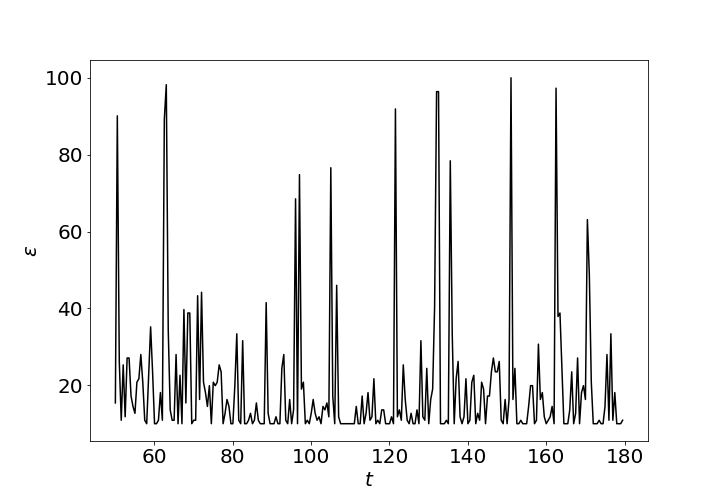
\includegraphics[width=6.5cm]{/Shape Parameter/Rossler t=180.png}&
                    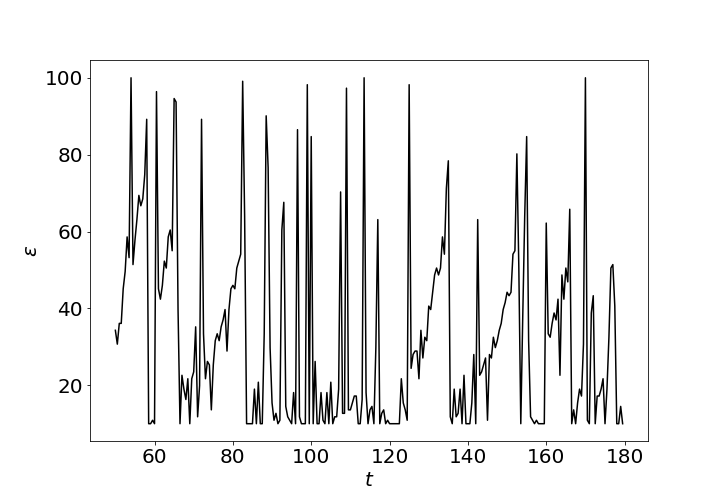
\includegraphics[width=6.5cm]{/Shape Parameter/Rossler t=180 dt=0,001.png}\\
                    \hfil a &b\\
                    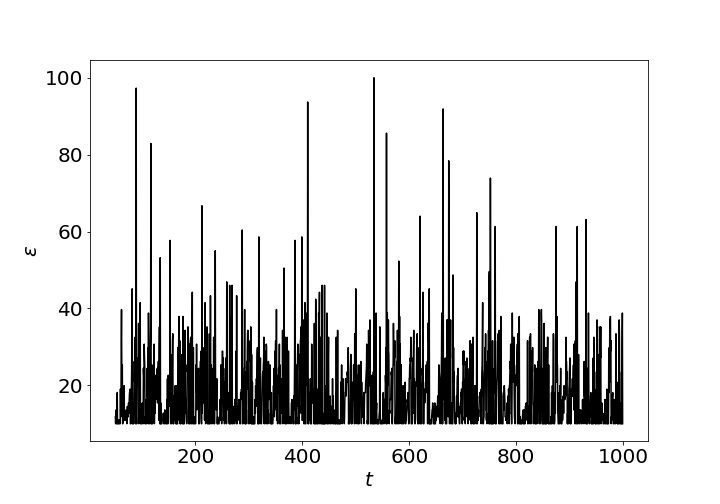
\includegraphics[width=6.5cm]{/Shape Parameter/Rossler t=1000.png}&
                    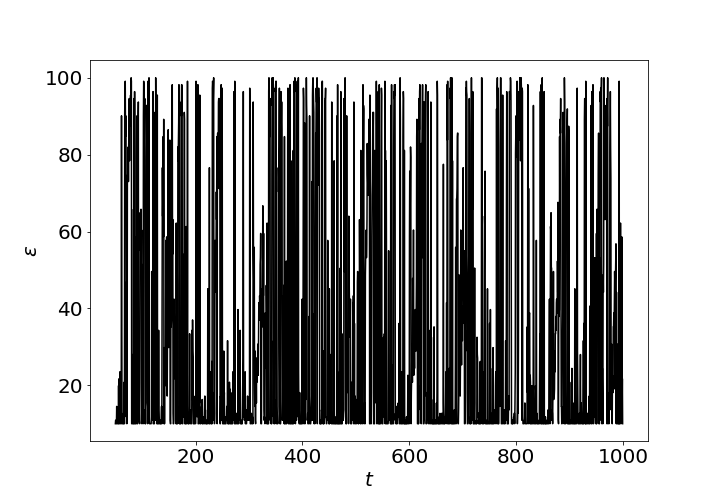
\includegraphics[width=6.5cm]{/Shape Parameter/Rossler t=1000 dt=0,001.png}\\
                    \hfil c &d\\
                \end{tabular}
                \caption{Rossler shape parameter vs time, a. $t=180$, $dt=0.01$ b. $t=180$, $dt=0.001$ c. $t=1000$, $dt=0.01$ d. $t=1000$, $dt=0.001$}\label{fig:rosslershape}
            \end{figure}
            \begin{figure}[H]
                \centering
                \begin{tabular}{lcc}
                    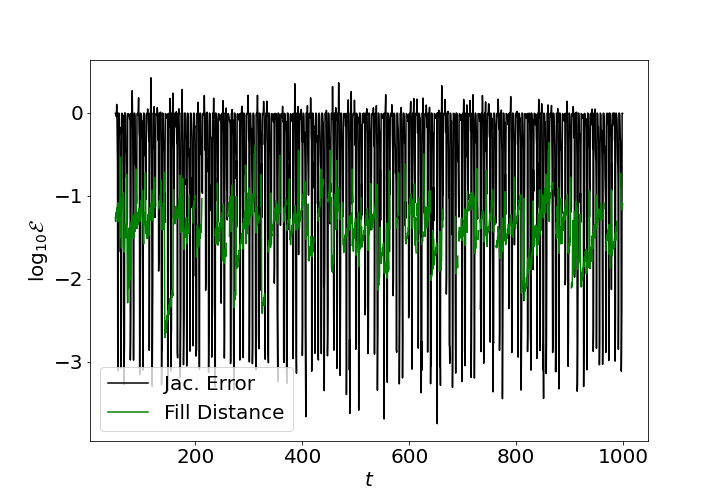
\includegraphics[width=6.5cm]{/Jacobian Error/Rossler mult.png}&
                    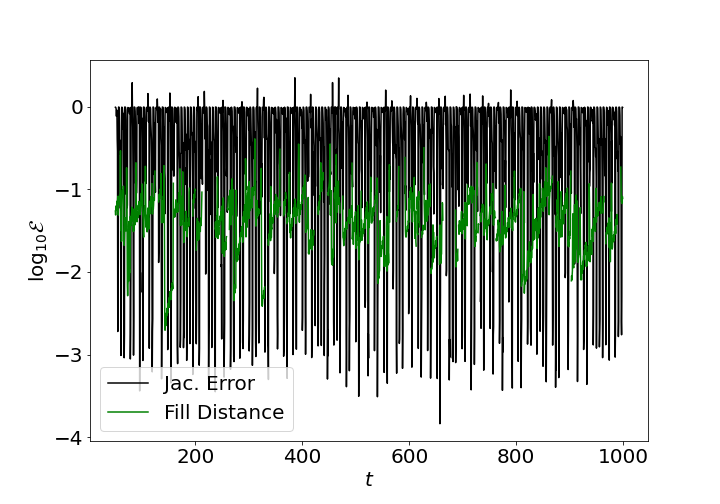
\includegraphics[width=6.5cm]{/Jacobian Error/Rossler inv.png}\\
                    \hfil a &b\\
                    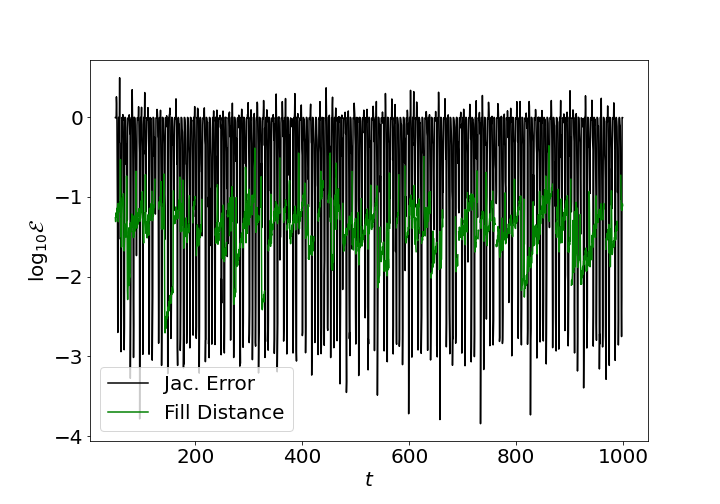
\includegraphics[width=6.5cm]{/Jacobian Error/Rossler, 100nbrs.png}&
                    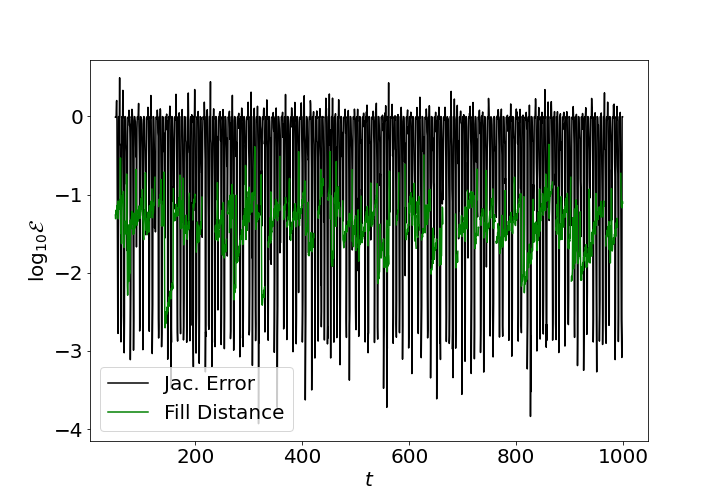
\includegraphics[width=6.5cm]{/Jacobian Error/Rossler, 150nbrs.png}\\
                    \hfil c &d\\
                \end{tabular}
                \caption{Rossler Jacobian Error and Fill Distance, a. $t=2000$, $dt=0.01$ b. $t=1000$, $dt=0.1$ c. $t=1000$, $dt=0.05$ d. $t=1000$, $dt=0.005$}\label{fig:rosslerjac3}
            \end{figure}

            \begin{table}
                \centering
                \begin{tabular}[h]{||c c c c c c c c||}
                    \hline
                    $\phi (x,\epsilon)$ & $t$ & $dt$ & $N_{nb}$ & $\lambda_1$ & $\lambda_2$ & $\lambda_3$ & $tr(\tilde{J}(t))$\\
                    \hline
                    gaussian & 180 & 0.01 & 50 & 0.0323797 & 0.00138742  &  -0.91939 & -0.8856\\
                    \hline
                    gaussian & 180 & 0.001 & 50 & 0.0290489 & 0.0011676 & -0.228423 & -0.1982\\
                    \hline
                    gaussian & 1000 & 0.01 & 50 & 0.0670752 & 0.000405778 &-1.69032 & -1.6228\\
                    \hline
                    gaussian & 2000 & 0.01 & 50 & 0.069549 & -0.000608606 &   -1.53759 & -1.4686\\
                    \hline
                    multiquadric & 1000 & 0.01 & 50 & 0.0670853 & 0.000419429 &   -1.6349 & -1.5674\\
                    \hline
                    inverse & 1000 & 0.01 & 50 & 0.0670964 & 0.000517378  &  -1.71732 & -1.6498\\
                    \hline
                    gaussian & 1000 & 0.01 & 100 & 0.0670358 & 0.000614184  &  -1.79644 & -1.7288\\
                    \hline
                    gaussian & 1000 & 0.01 & 150 & 0.0669915 & 0.000366926  &  -1.66476 & -1.5974\\
                    \hline
                    gaussian & 1000 & 0.1 & 50 & 0.0559489 & -0.0302194  &  -2.59748 & -2.5718\\
                    \hline
                    gaussian & 1000 & 0.05 & 50 & 0.0695828 & -0.00497013   & -1.95738 & -1.8928\\
                    \hline
                    gaussian & 1000 & 0.005 & 50 & 0.0660092 & -8.18815e-05  &  -1.44486 & -1.3789\\
                    \hline
                    gaussian & 1000 & 0.001 & 50 & 0.0687768 & -0.000587808  &  -1.06623 & -0.9980\\ [1ex]
                    \hline
                \end{tabular}\\
                \caption{MSDI-RBF Lyapunov Estimates for Rossler equation}\label{table:rosslerest}
            \end{table}

        \section{Chua and Li Attractors}

                The Chua equation and Li equation were tested using the three basic functions presented in this thesis. In both systems,
                $t=1000$,  $dt=0.01$, and $N_{nb}=50$. The Lyapunov
                exponent estimations for Chua and Li can be found in Tables \ref{table:chuaest} and \ref{table:liest} respectively.\\
                \begin{table}
                    \centering
                    \begin{tabular}[h]{||c c c c c c c c||}
                        \hline
                        $\phi (x,\epsilon)$ & $t$ & $dt$ & $N_{nb}$ & $\lambda_1$ & $\lambda_2$ & $\lambda_3$ & $tr(\tilde{J}(t))$ \\
                        \hline
                        gaussian & 1000 & 0.01 & 50 & 0.380541 & -0.0169871  &  -2.59346 & -2.2299\\
                        \hline
                        multiquadric & 1000 & 0.01 & 50 & 0.384737 & -0.0261238 &   -2.61506 & -2.2564\\
                        \hline
                        inverse & 1000 & 0.01 & 50 & 0.412058 & 0.000260987 &   -2.58251 & -2.1702\\ [1ex]
                        \hline
                    \end{tabular}\\
                    \caption{MSDI-RBF Lyapunov Estimates for Chua equation}\label{table:chuaest}
                \end{table}
                \begin{table}
                    \centering
                    \begin{tabular}[h]{||c c c c c c c c||}
                        \hline
                        $\phi (x,\epsilon)$ & $t$ & $dt$ & $N_{nb}$ & $\lambda_1$ & $\lambda_2$ & $\lambda_3$ & $tr(\tilde{J}(t))$ \\
                        \hline
                        gaussian & 1000 & 0.01 & 50 & 0.565762 & -0.0335047  &  -1.45285 & -0.9206\\
                        \hline
                        multiquadric & 1000 & 0.01 & 50 & 0.536935 & -0.0137958  &  -1.45266 & -0.9295\\
                        \hline
                        inverse & 1000 & 0.01 & 50 & 0.515629 &  0.0192148  &  -1.52953 & -0.9947\\ [1ex]
                        \hline
                    \end{tabular}\\
                    \caption{MSDI-RBF Lyapunov Estimates for Li equation}\label{table:liest}
                \end{table}

\chapter{Discussion}

    In Table \ref{table:deici} we see significant variation in the results to the test algorithm. This is seen strongly
    in $\lambda_2$ for Lorenz where at $dt=0.1$ $\lambda_2\approx 0.17$ but at $dt=0.001$ $\lambda_2\approx 0.004$. However,
    we do see convergent behavior as we decrease the time step of this algorithm when comparing the results the results
    to the literature (Table \ref{table:lit}). Therefore we can conclude that the test algorithm is a good metric to compare
    MSDI-RBF against.\\

            The results from Lorenz are promising and suggest that we can trust the Lyapunov exponent
            approximations produced by the MSDI-RBF scheme for the Lorenz equations. Comparing Figure \ref{fig:lorenzjac} to Figure \ref{fig:lorenzshape} we see that the shape parameter $\epsilon$ is more responsive to moving along
            the trajectory than the fill distance in respect to the Jacobian error. We see that the optimal shape parameter
            is erratic with respect to time. The shape parameter allows the RBF to adapt as the data set evolves in
            time and the behavior in Figure \ref{fig:lorenzshape} explains the ability of the RBF to adapt to changing conditions keeping the overall relative error
            of the Jacobian approximations small. This result tells us that RBFs give us
            a straightforward and accurate means of approximating Jacobians along a flow.\\

            The choice of a time step for the Runge-Kutta scheme has a strong impact on the accuracy of the MSDI-RBF scheme
            for the Lorenz equation. In Figure \ref{fig:lorenzjac}a we can see a minimum error around the order of -2.5.
            However, in Figure \ref{fig:lorenzjac}b we see errors on the order of -3. However, we also see periodic order one errors. The associated
            shape parameter in Figure \ref{fig:lorenzshape}b also appears less dynamic, with most values $<40$ with rare and drastic spikes
            interspersed. We see the result of these errors and lack of adaptability in Table \ref{table:lorenzest} for
            the trial $t=90, \ \dt=0.001$ as the minimal Lyapunov exponent is inaccurate. This is a manifestation of the
            accuracy vs. stability trade off principle. The length of the simulation run time also
            seems to have an impact on on the accuracy of the scheme but its contribution is dwarfed by the time step. We can
            see that this is the case in Figure \ref{fig:lorenzjac}c as the order of error barely exceeds -2.5, giving us
            less accuracy than the significantly shorter simulation run time presented in Figure \ref{fig:lorenzjac}b. Additionally,
            In Figure \ref{fig:lorenzjac}d the error decreases by a magnitude from Figure \ref{fig:lorenzjac}b reaching an order of
            -4 demonstrating that simulation run time has a stronger impact the finer the data is.\\

            While the maximal Lyapunov exponent of $t=90, \ dt=0.001$ is on par with $t=1000, \ dt=0.01$ (Table \ref{table:lorenzest}), the smallest
            Lyapunov exponent of the latter is more accurate according to Table \ref{table:deici} and results that are
            found in the literature (Table \ref{table:lit}). This suggests that the length of the simulation run time may have a
            greater role to play in the accuracy of the smallest Lyapunov exponent. As stated previously, we can see the order of error jump periodically
            to order one in Figure \ref{fig:lorenzjac}b. These moments of
            high error contribute to the higher degree of inaccuracy for the smallest Lyapunov exponent. These periodic jumps seem to lessen
            as we increase the time length (Figure \ref{fig:lorenzjac}d).
            It is likely that both of the aformentioned parameters have a role to play in the accuracy of the minimal
            Lyapunov exponent as we see convergence in the minimal exponent for $t=1000, \ dt=0.001$.\\

            Turning our attention to
            Rossler, the Jacobian errors behave very differently from what
            we saw for the Lorenz Jacobian errors. Rossler's Jacobian errors have periodic order one reoccurances with strong, but rare,
            radical departures. The Jacobian errors for Rossler do not seem well correlated to the fill distance, suggesting
            that the problem lies in the centered difference approximation underlying the interpolation scheme. As can be seen
            in Figure \ref{fig:rosslershape}, the shape parameter appears less adaptive than what we see with Lorenz. Rossler
            has strong temporal gradients due to a nearly singular perturbative phenomenon in its dynamics. This manifests
            as stiffness in our algorithm.\\

            Figure \ref{fig:rosslerjac} lends some evidence to the aforementioned hypothesis. Looking at Figure \ref{fig:rosslerjac}a,
            we can see that this experiment yielded minimum Jacobian errors on the order of -3 while Figure \ref{fig:rosslerjac}b yielded
            minimal errors on the order of -2. If we look at the corresponding data in Table \ref{table:rosslerest}, $t=180, \ dt=0.01$
            and $t=180, \ dt=0.001$ respectively, the latter's maximal Lyapunov exponent is less accurate than the former's
            according to Table \ref{table:deici}. In Figure \ref{fig:rosslerjac}c and d we see that the minimal Jacobian errors
            reach the order of -4 (with one spike reaching -5 in Figure \ref{fig:rosslerjac}d). Referring back to Table \ref{table:rosslerest}
            we can see convergent behavior of the maximal Lyapunov exponent with respect to Table \ref{table:deici} and the
            literature \cite{item:8}. Additionally, we can see similar behavior in the minimal Lyapunov exponent for Rossler
            generally and $t=180, \ dt=0.001$ in Table \ref{table:lorenzest}.\\

            We conducted trials both Rossler and Lorenz measuring the effect of increasing the number of nearest nearest
            neighbors on the Jacobian error and Lyapunov estimates (Figures \ref{fig:lorenzjac3} and \ref{fig:rosslerjac3}). However, the
            effect the number of nearest neighbors has in this range seems negligible on the Jacobian error. Multiquadric and inverse basic
            functions also appear to have a
            negligible effect on our estimates (Figures \ref{fig:lorenzjac3} and \ref{fig:rosslerjac3}).
            The Lyapunov exponent estimates for both systems are presented in Table \ref{table:lorenzest} and \ref{table:rosslerest}.\\


            The trials for the Chua and Li equations were not as extensive in scope as Lorenz and Rossler.
            The Chua and Li attractors share similar geometry with the Lorenz attractor and as such we can hypothesize that they will have
            similar performance with the MSDI-RBF algorithm. This hypothesis is confirmed by the Lyapunov exponent estimates of Chua and presented in Table \ref{table:chuaest}
            and of Li in Table \ref{table:liest}. These results demonstrate the effectiveness of the MSDI-RBF algorithm for attractors
            beyond Lorenz. For both systems we have similar results to the Lyapunov exponents calculated for these systems
            in Table \ref{table:deici} as well as what is presented in the literature (Table \ref{table:lit}).\\
            \begin{table}
                    \centering
                    \begin{tabular}[h]{||c c c c||}
                        \hline
                        system & $\lambda_1$ & $\lambda_2$ & $\lambda_3$ \\
                        \hline
                        Lorenz \cite{item:8} & 9.056 & 0  &  -14.5723\\
                        \hline
                        Rossler \cite{item:8} & 0.0714 & 0  &  -5.3943\\
                        \hline
                        Chua \cite{item:8} & 0.3271 &  0  &  -2.5197\\
                        \hline
                        Li \cite{item:6} & 0.131 & 0 & 1.131\\[1ex]
                        \hline
                    \end{tabular}\\
                    \caption{Lyapunov exponents for systems from literature}\label{table:lit}
                \end{table}

\chapter{Conclusion}

            This thesis has shown that the MSDI-RBF method is a promising method for the estimation of Lyapunov exponents.
            The method offers a globally convergent data driven method for calculating Lyapunov exponents of dynamical systems,
            but there are situations where the scheme struggled. The Lorenz estimates for finer time steps $t=1000, \ dt=0.005, \ \dt=0.001$
            gave accurate estimates of the Lyapunov exponent. The estimates for Chua are very good. Li's Lyapunov estimates are less accurate.
            However, based on what we see in Table \ref{table:lorenzest} for the trials where $t=1000, \ dt=0.01, \ N_{nb}=50$,
            we can infer that Li would benefit from an improved time step. It is encouraging that the trials for these attractors
            yielded results similar to what can be seen in the literature (see Table \ref{table:lit}).\\

            Singularly perturbed flows such as Rossler suffer from
            stiffness in the algorithm causing inaccurate results.
            Additionally, there is some evidence that fine data collected over too short of an amount of time may yield inaccurate
            results particular in respect to the minimal Lyapunov exponent as we see in Table \ref{table:lorenzest} for trial $t=90, \ dt=0.001$. However, the maximal Lyapunov exponent seems
            easier for MSDI-RBF to discern even for difficult attractors such as Rossler. The MSDI-RBF algorithm can then
            be used to firmly establish the presence of chaos in a dynamical system.\\

            Centered finite differencing is based on Taylor
            series expansions and as such are locally convergent and may introduce errors. A topic
            of future work may be to develop an RBF scheme, or use other numerical differentiation methods, to generate the initial approximation of points in the unknown function $\mathbf{f}(\mathbf{y})$
            instead of relying on finite differencing methods.\\

            Preconditioning may help to produce more accurate of singularly perturbed systems. Recently, machine learning has
            been utilized to study dynamical systems. There is a family of techniques that utilize the Koopman operator called
            Dynamic Mode Decomposition (DMD). The Koopman operator allows one to take complicated nonlinear dynamics and
            put them into a space where they appear linear. Recent work by \textit{Curtis et al.} \cite{item:10} and \textit{Gilpin}
            \cite{item:20} use autoencoders to achieve this. Use of such techniques may allow one to take ill-behaved systems
            and put them in a space where the MSDI-RBF algorithm is easier to work with.\\

            Once accurate results for the Rossler equation can be obtained with an improved MSDI-RBF procedure. The improved
            scheme should be tested with the Rabinovich-Fabrikant equation across different equation parameters. The
            Rabinovich-Fabrikant equation is a dynamical system also capable of chaotic behavior. Changing the equation
            parameters of this system can radically alter the geometry of the attractor.
            an attractor of similar singularly perturbed geometry that Rossler exhibits \cite{item:8}. Additionally, the same equation parameter
            This equation is capable of producing different attractors by using different time steps in the numerical integrator \cite{item:22}.
            The difficulty of this equation would provide a good stress test to an improved MSDI-RBF in future work.\\

    \nocite{*}
    \bibliographystyle{siammod}
    \bibliography{thbib}
    \appendix
%
% If you only have one appendix, you should change the above to:
%\appendix
%

\chapter{}

\begin{figure}[H]
    \centering
    \begin{tabular}{lcc}
        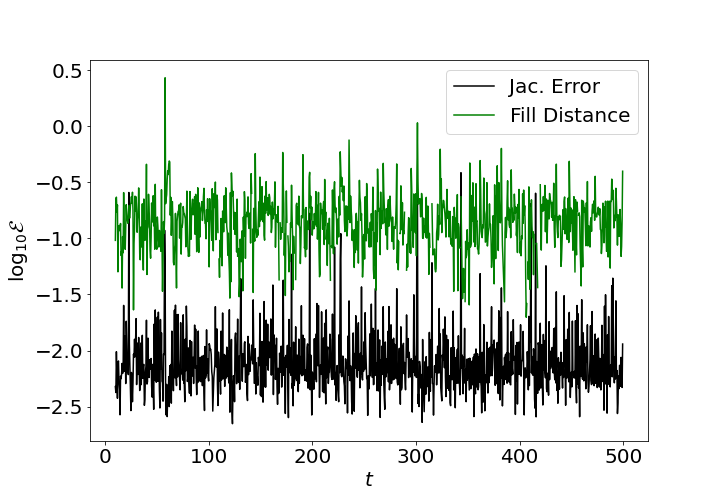
\includegraphics[width=6.5cm]{/Jacobian Error/Lorenz, t=500.png}&
        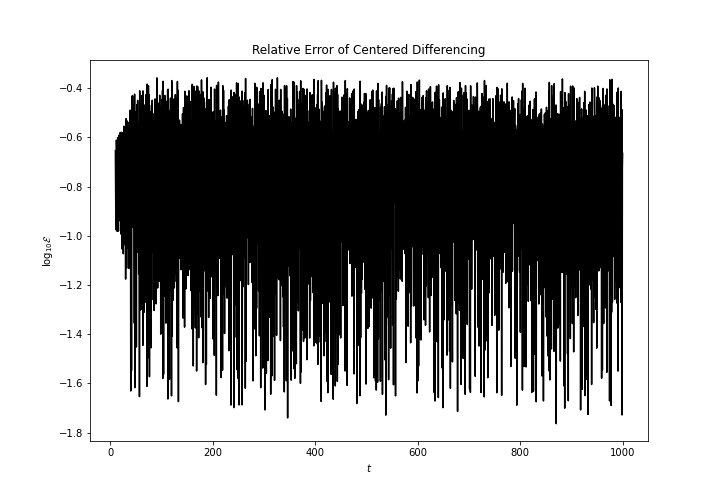
\includegraphics[width=6.5cm]{/Jacobian Error/Lorenz, dt=0,1.png}\\
        \hfil a &b\\
        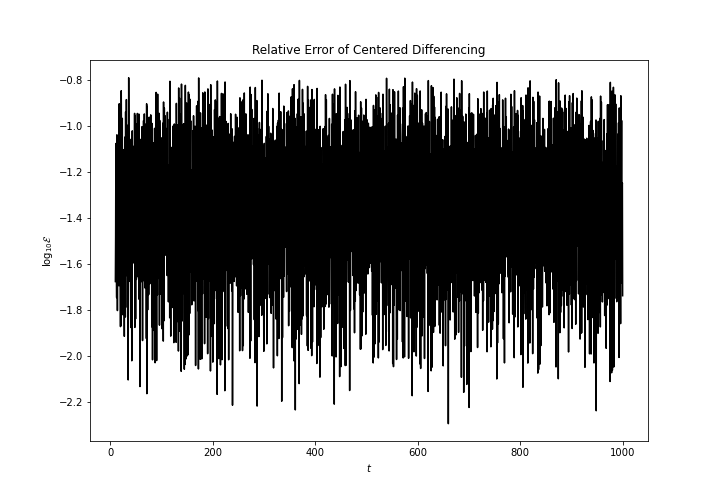
\includegraphics[width=6.5cm]{/Jacobian Error/Lorenz, dt=0,05.png}&
        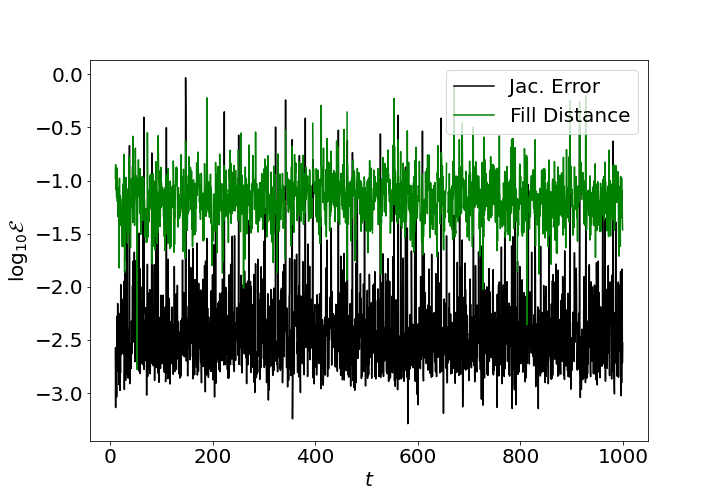
\includegraphics[width=6.5cm]{/Jacobian Error/Lorenz, dt=0,005.png}\\
        \hfil c &d\\
    \end{tabular}
    \caption{Lorenz Jacobian Error and Fill Distance, a. $t=500$, $dt=0.01$ b. $t=1000$, $dt=0.1$ c. $t=1000$, $dt=0.05$ d. $t=1000$, $dt=0.005$}\label{fig:lorenzjac2}
\end{figure}

\begin{figure}[H]
    \centering
    \begin{tabular}{lcc}
        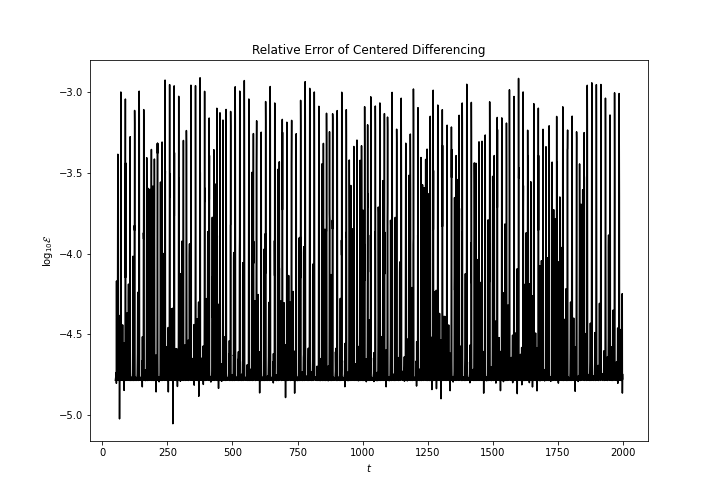
\includegraphics[width=6.5cm]{/Jacobian Error/Rossler, t=2000.png}&
        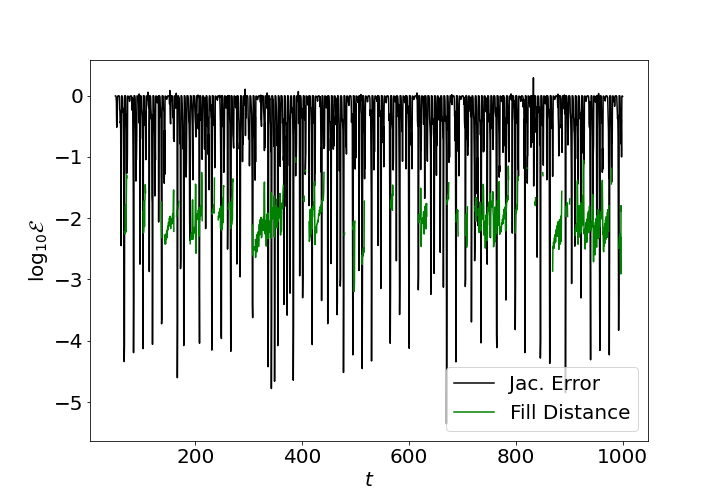
\includegraphics[width=6.5cm]{/Jacobian Error/Rossler, dt=0,1.png}\\
        \hfil a &b\\
        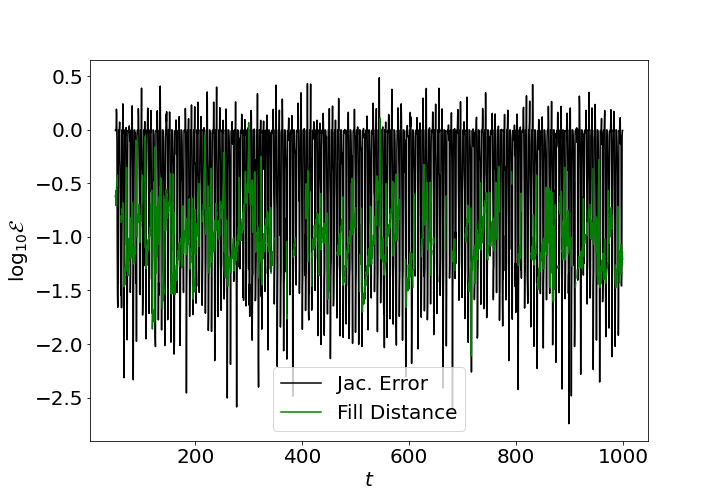
\includegraphics[width=6.5cm]{/Jacobian Error/Rossler, dt=0,05.png}&
        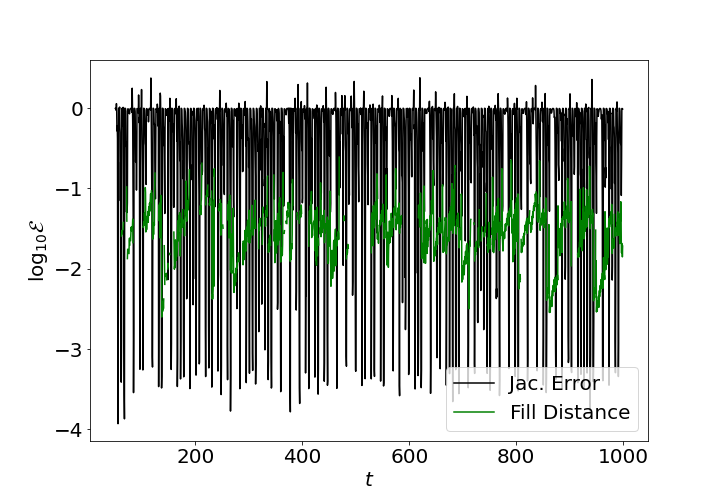
\includegraphics[width=6.5cm]{/Jacobian Error/Rossler, dt=0,005.png}\\
        \hfil c &d\\
    \end{tabular}
    \caption{Rossler Jacobian Error and Fill Distance, a. $t=2000$, $dt=0.01$ b. $t=1000$, $dt=0.1$ c. $t=1000$, $dt=0.05$ d. $t=1000$, $dt=0.005$}\label{fig:rosslerjac2}
\end{figure}


\end{document}